% !TeX spellcheck = it_IT
\title{Informatica Teorica}
\author{Massimo Perego, Omar Masri}
\date{}

\documentclass[11pt]{report}
\usepackage[paperwidth=330mm, paperheight=297mm, left=2cm, top=2cm, bottom=2cm, right=14cm, marginparsep=1cm, marginparwidth=12cm]{geometry}
\usepackage{graphicx} 
\usepackage{amsmath}
\usepackage{amssymb}
\usepackage{amsfonts}
\usepackage[hidelinks]{hyperref}
\usepackage[american]{babel}
\usepackage[autostyle, english = american]{csquotes}
\usepackage[parfill]{parskip}
\MakeOuterQuote{"}

\usepackage{dutchcal}
\usepackage{tikz}
\usetikzlibrary{shapes,arrows,positioning, intersections, calc}
\usepackage{amsthm}
\usepackage{array}
\usepackage{calc}
\newcolumntype{C}[1]{wc{\widthof{#1}}} % fixed width & centered
\usepackage{ifthen}
\usepackage{stmaryrd}
\usepackage{multirow}
\usepackage{mathtools}
\usepackage[italiano,noline]{algorithm2e}
\usepackage{tcolorbox}
\usepackage{setspace}
\usepackage{amsthm}
\usepackage{mathabx}
\usepackage{bm}
\usepackage{minted}
\usepackage{xcolor}
\definecolor{bg}{rgb}{0.95,0.95,0.95}
\setminted[python]{linenos, bgcolor=bg}

\theoremstyle{plain}
\newtheorem{theor}{Teorema}[section]
\newtheorem{coroll}{Corollario}[section]

\renewcommand{\proofname}{Dimostrazione}

\DeclareMathOperator{\des}{des}
\DeclareMathOperator{\op}{op}
\DeclareMathOperator{\somma}{somma}
\DeclareMathOperator{\prodotto}{prodotto}
\DeclareMathOperator{\predecessore}{predecessore}
\DeclareMathOperator{\MIN}{MIN}

\usepackage{marginnote}
\newcommand{\lcomment}[1]{\marginnote{$\leftarrow$ (#1)}}
\usepackage[noend]{algpseudocode}

\renewcommand{\Im}{\text{Im}}
\newcommand{\ImSet}{\text{Im}}
\newcommand{\Dom}{\text{Dom}}
\newcommand{\tc}{\; \text{ t.c. } \;}
\newcommand{\bat}{B^A_\bot}
\newcommand{\dati}{\text{DATI}}
\newcommand{\prog}{\text{PROG}}
\newcommand{\dtime}{\text{DTIME}}
\newcommand{\ftime}{\text{FTIME}}
\newcommand{\dspace}{\text{DSPACE}}
\newcommand{\fspace}{\text{FSPACE}}
\newcommand{\exptime}{\text{EXPTIME}}
\newcommand{\ntime}{\text{NTIME}}
\newcommand{\ram}{\text{RAM}}
\newcommand{\while}{\text{WHILE}}
\newcommand{\for}{\text{FOR}}
\newcommand{\stati}{\text{STATI}}
\newcommand{\elem}{\text{ELEM}}
\newcommand{\elemo}{\text{ELEM}^\Omega}
\newcommand{\wstati}{W\text{-STATI}}
\newcommand{\wcom}{W\text{-COM}}
\newcommand{\wprog}{W\text{-PROG}}
\newcommand{\comp}{\text{Comp}}
\newcommand{\com}{\text{COMP}}
\newcommand{\rp}{\text{RP}}
\newcommand{\pc}{\text{PC}}
\newcommand{\ricprim}{\text{RICPRIM}}
\newcommand{\ric}{\text{RIC}}
\newcommand{\C}{\mathcal{C}}
\newcommand{\U}{\mathcal{U}}
\newcommand{\cp}{\mathcal{P}}
\newcommand{\st}{\mathcal{S}}
\newcommand{\T}{\mathcal{T}}
\newcommand{\N}{\mathbb{N}}
\newcommand{\R}{\mathbb{R}}
\newcommand{\X}{\mathcal{X}}
\newcommand{\cprog}[1]{\C_{#1}\text{-}\prog}
\newcommand{\proj}{\text{Proj}}
\newcommand{\pro}{\text{Pro}}
\newcommand{\incr}{\text{incr}}
\newcommand{\decr}{\text{decr}}
\newcommand{\sisprog}{\ensuremath{\{\varphi_i\}}}
\newcommand{\fin}{\stackrel{\text{TR}}{=} \text{OK}}
\newcommand{\ar}{\text{AR}}
\newcommand{\arp}{\text{AR}_P}
\newcommand{\arph}{\text{AR}_{\hat{P}}}
\newcommand{\cent}{\text{\textcent}}

\newcommand{\si}{\textit{Sì}}
\newcommand{\no}{\textit{No}}

\newcommand{\dotminus}{\dotdiv}

\makeatletter
\renewcommand{\@chapapp}{Capitolo}
\renewcommand{\contentsname}{Indice}
\makeatother

\begin{document}
	
	\tikzstyle{block} = [draw, rectangle, minimum height=2em, minimum width=3em]
	
	\maketitle
	\tableofcontents
	\newpage
	
	% !TeX spellcheck = it_IT
% !TeX root = ../it.tex

\chapter*{Introduzione}
\addcontentsline{toc}{chapter}{Introduzione}

Si "contrappone" all'informatica applicata, ovvero qualsiasi applicazione dell'informatica atta a raggiunger uno scopo, dove l'informatica è solamente lo strumento per raggiungere in maniera efficace un obiettivo.\\
Con "\textit{informatica teorica}" l'oggetto è l'informatica stessa, si studiano i fondamenti della disciplina in modo rigoroso e scientifico. Può essere fatto ponendosi delle questioni fondamentali: il \textit{cosa} e il \textit{come} dell'informatica, ovvero cosa è in grado di fare l'informatica e come è in grado di farlo.

\paragraph{Cosa:} L'informatica è "la disciplina che studia l'informazione e la sua elaborazione automatica", quindi l'oggetto sono l'informazione e i dispositivi di calcolo per gestirla; scienza dell'informazione. Diventa lo studio come risolvere automaticamente un problema. Ma tutti i problemi sono risolvibili in maniera automatica? Cosa è in grado di fare l'informatica? \\

La branca dell'informatica teorica che studia cosa è risolvibile si chiama \textbf{Teoria della Calcolabilità}, studia cosa è calcolabile per via automatica. Spoiler: non tutti i problemi sono risolvibili per via automatica, e non potranno mai esserlo per limiti dell'informatica stessa. Cerchiamo una caratterizzazione generale di cosa è calcolabile e cosa no, si vogliono fornire strumenti per capire ciò che è calcolabile. La caratterizzazione deve essere fatta matematicamente, in quanto il rigore e la tecnica matematica permettono di trarre conclusioni sull'informatica.

\paragraph{Come:} Una volta individuati i problemi calcolabili, come possiamo calcolarli? Il dominio della \textbf{Teoria della Complessità} vuole descrivere le risoluzione dei problemi tramite mezzi automatici in termini di risorse computazionali necessarie. Una "risorsa computazionale" è qualsiasi cosa che viene consumata durante l'esecuzione per risolvere il problema, come possono essere elettricità o numero di processori, generalmente i parametri più importanti considerati sono tempo e spazio di memoria. Bisognerà definire in modo preciso cosa si intende con "tempo" e "spazio". Una volta fissati i parametri bisogna definire anche cosa si intende con "risolvere efficientemente" un problema, in termini di tempo e spazio.\\

La teoria della calcolabilità dice quali problemi sono calcolabili, la teoria della complessità dice, all'interno dei problemi calcolabili, quali sono risolvibili efficientemente.\\
	
	% !TeX spellcheck = it_IT
% !TeX root = ../it.tex

\chapter{Teoria della Calcolabilità}

\section{Notazione}

\subsection{Funzioni}

\paragraph{Funzione:} Una funzione $f$ dall'insieme $A$ all'insieme $B$ è una legge che dice come associare a ogni elemento di $A$ un elemento di $B$. Si scrive
$$ f: A \rightarrow B $$
E chiamiamo $A$ dominio e $B$ codominio. Per dire come agisce su un elemento si usa $f(a) = b$, $b$ è l'immagine di $a$ secondo $f$ (di conseguenza $a$ è la controimmagine).\\
Per definizione di funzione, è possibile che elementi del codominio siano raggiungibili da più elementi del dominio, ma non il contrario. Possiamo classificare le funzioni in base a questa caratteristica:
\begin{itemize}
	\item \textbf{Iniettiva:} $f: A \rightarrow B$ è iniettiva sse $\forall a,b \in A$, $a \neq b \implies f(a) \neq f(b)$
	\item \textbf{Suriettiva:} $f: A \rightarrow B$ è suriettiva sse $\forall b \in B$, $\exists a \in A: f(a) = b$: un altro modo per definirla è tramite l'insieme immagine di $f$, definito come
	$$ \ImSet_f = \{b \in B: \exists a, f(a) = b \} = \{f(a): a \in A \} $$
	Solitamente $\text{Im}_f \subseteq B$, ma $f$ è suriettiva sse $ \ImSet_f = B$;
	\item \textbf{Biettiva:} $f: A \rightarrow B$ è biettiva sse è sia iniettiva che suriettiva, ovvero
	$$
	\begin{array}{c l}
		\forall a, b \in A, a \neq b: & f(a) \neq f(b) \\
		\forall b \in B, \exists a \in A: & f(a) = b
	\end{array}
	\implies \forall b \in B, \exists! a \in A: f(a) = b
	$$
\end{itemize}

\paragraph{Inversa:} Per le funzioni biettive si può naturalmente associare il concetto di "inversa": dato $f: A \rightarrow B$ biettiva, si definisce inversa la funzione $f^{-1}: B \rightarrow A$ tale che $f^{-1} (b) = a \Leftrightarrow f(a) = b$.\\

\paragraph{Composizione di funzioni:} Date $f: A \rightarrow B$ e $g: B \rightarrow C$, $f$ composto $g$ è la funzione $g \circ f: A \rightarrow C$ definita come $g \circ f(a) = g(f(a))$. Generalmente non commutativo, $f \circ g \neq g \circ f$, ma è associativo.\\

\paragraph{Funzione identità:} Dato l'insieme $A$, la funzione identità su $A$ è la funzione $i_A: A \rightarrow A$ tale che $i_A (a) = a$, $\forall a \in A$.\\

Un'altra possibile definizione per l'inversa diventa:
$$ f^{-1} \circ f = i_A \wedge f \circ f^{-1} = i_B $$

\paragraph{Funzioni Parziali:} Se una funzione $f: A \rightarrow B$ è definita per $a \in A$ si indica con $f(a) \downarrow$ e da questo proviene la categorizzazione: una funzione è \textbf{totale} se definita $\forall a \in A$, \textbf{parziale} altrimenti (definita solo per qualche elemento di $A$).\\

\paragraph{Insieme Dominio:} Chiamiamo \textbf{dominio} (o campo di esistenza) di $f$ l'insieme
$$ \Dom_f = \left\{a \in A | f(a) \downarrow \right\} \subseteq A $$
Quindi se $\Dom_f = A$ la funzione è totale, se $\Dom_f \subsetneq A$ allora è una funzione parziale.\\

\paragraph{Totalizzazione:} Si può \textbf{totalizzare una funzione parziale} $f$ definendo una funzione a tratti $\overline{f}: A \rightarrow B \cup \{\bot\}$ tale che
$$ 
\overline{f} (a) = \begin{cases}
	f(a) & a \in \Dom_f(a) \\
	\bot & \text{altrimenti}
\end{cases}
$$
Dove $\bot$ è il \textbf{simbolo di indefinito}, per tutti i valori per cui la funzione di partenza $f$ non è definita. Da qui in poi $B_\bot$ significa $B \cup \{\bot\}$.\\

\paragraph{Insieme delle funzioni:} L'insieme di tutte le funzioni che vanno da $A$ a $B$ si denota con
$$ B^A = \{f: A \rightarrow B \} $$
La notazione viene usata in quanto la cardinalità di $B^A$ è esattamente $|B|^{|A|}$, con $A$ e $B$ insiemi finiti.\\
Volendo includere anche tutte le funzioni parziali: 
$$ B^A_\bot = \{f: A \rightarrow B_\bot \} $$
Le due definizioni coincidono, $B^A = B^A_\bot$, ma quest'ultima permette di mettere in evidenza che tutte le funzioni presenti sono totali o totalizzate.\\ 

\subsection{Prodotto Cartesiano}

Chiamiamo \textbf{prodotto cartesiano} l'insieme 
$$ A \times B = \{(a,b) | a \in A \wedge b \in B \} $$
Rappresenta l'insieme di tutte le coppie ordinate di valori in $A$ e $B$. In generale non è commutativo, a meno che $A=B$.\\

Può essere esteso a $n$-uple di valori:
$$ A_1 \times \dots \times A_n = \{(a_1, \dots, a_n) | a_i \in A_i\} $$
Il prodotto di $n$ volte lo stesso insieme verrà, per comodità, indicato come
$$ A \times \dots \times A = A^n $$

\paragraph{Proiettore:} Operazione "opposta", il proiettore $i$-esimo è una funzione che estrae l'$i$-esimo elemento di una tupla, quindi è una funzione
$$ \pi_i: A_1 \times \dots \times A_n \rightarrow A_i \tc \pi_i (a_1, \dots, a_n) = a_i $$
La proiezione sull'asse in cui sono presenti i valori dell'insieme $a_i$.\\

\subsection{Funzione di Valutazione}
Dati $A,B$ e $B^A_\bot$ si definisce \textbf{funzione di valutazione} la funzione
$$ \omega: \bat \times A \rightarrow B \tc \omega (f,a) = f(a) $$
Prende una funzione $f$ e la valuta su un elemento $a$ del dominio. Si possono fare due tipi di analisi su questa funzione: 
\begin{itemize}
	\item Fisso $a$ e provo tutte le $f$, ottenendo un \textit{benchmark} di tutte le funzioni su $a$
	\item Fisso $f$ e provo tutte le $a$ del dominio, ottenendo il \textit{grafico} di $f$
\end{itemize}

\section{Sistemi di Calcolo}

Vogliamo modellare teoricamente un \textbf{sistema di calcolo}; quest'ultimo può essere visto come una black box che prende in input un programma $P$, dei dati $x$ e calcola il risultato $y$ di $P$ su input $x$. La macchina restituisce $y$ se è riuscita a calcolare un risultato, $\bot$ (indefinito) se è entrata in un loop.
\begin{center}
	\begin{tikzpicture}[>=stealth, auto, node distance=2cm]
		\node [block] (C) { Calcolatore };
		\node [left=of C.west, below] (P)  {$P$};
		\node [left=of C.west, above] (x)  {$x$};
		\node [right=of C] (out)  {$y/\bot$};
		
		\draw [->] (x) -- node {} (C.169);
		\draw [->] (P) -- node {} (C.194);
		\draw [->] (C) -- node {} (out);
\end{tikzpicture}

\end{center}

Quindi, formalmente, possiamo definire un sistema di calcolo come una funzione 
$$ \C: \prog \times \dati \rightarrow \dati_\bot $$

Possiamo vedere un sistema di calcolo come una funzione di valutazione:
\begin{itemize}
	\item i dati $x$ corrispondono all'input $a$
	\item il programma $P$ corrisponde alla funzione $f$
\end{itemize}

Formalmente, un programma $P \in \prog$ è una sequenza di regole che trasformano un dato input in uno di output, ovvero l'espressione di una funzione secondo una sintassi 
$$ P: \dati \rightarrow \dati_\bot $$
e di conseguenza $P \in \dati^{\dati}_\bot$. In questo modo abbiamo mappato l'insieme $\prog$ sull'insieme delle funzioni, il che ci permette di definire il sistema di calcolo come la funzione
$$ \C: \dati^{\dati}_\bot \times \dati \rightarrow \dati $$

Analoga alla funzione di valutazione. Con $\C(P,x)$ indichiamo la funzione calcolata da $P$ su $x$ dal sistema di calcolo $\C$, che viene detta \textbf{semantica}, ovvero il suo "significato" su input $x$.\\

Il modello solitamente considerato quando si parla di calcolatori è quello di \textbf{Von Neumann}.\\

\section{Potenza Computazionale}
Indicando con 
$$ \C (P, \_): \dati \rightarrow \dati $$
la funzione che viene calcolata dal programma $P$ (semantica di $P$).\\

La \textbf{potenza computazionale} di un calcolatore è definita come l'insieme di tutte le funzioni che quel sistema di calcolo è in grado di calcolare, ovvero
$$ F(\C) = \{\C (P, \_) | P \in \prog\} \subseteq \dati_\bot^{\dati} $$

Ovvero, l'insieme di tutte le possibili semantiche di funzioni calcolabili con il sistema $\C$. Stabilire il carattere di quest'ultima inclusione equivale a stabilire \textit{cosa può fare l'informatica}:
\begin{itemize}
	\item se $F(\C) \subsetneq \dati_\bot^{\dati}$ allora esistono compiti \textbf{non automatizzabili}
	\item se $F(\C) = \dati_\bot^{\dati}$ allora l'informatica \textit{può fare tutto}
\end{itemize}

Calcolare funzioni vuol dire risolvere problemi \textit{in generale}, a ogni problema è possibile associare una funzione soluzione che permette di risolverlo automaticamente.\\

Un possibile approccio per risolvere l'inclusione è tramite la \textbf{cardinalità} (funzione che associa ogni insieme al numero di elementi che contiene) dei due insiemi. Potrebbe però presentare dei problemi: è efficace solo quando si parla di insiemi finiti. Ad esempio, l'insieme dei numeri naturali contiene l'insieme dei numeri pari $\mathbb{P} \subsetneq \mathbb{N}$, ma $|\mathbb{N}| = |\mathbb{P}| = \infty$.\\
Serve una diversa definizione di cardinalità che considera l'esistenza di infiniti \textit{più densi di altri}.\\

\section{Relazioni di Equivalenza}
Dati due insiemi $A,B$, una relazione binaria $R$ è un sottoinsieme $R \subseteq A \times B$ di coppie ordinate. Data $R \subseteq A^2$, due elementi sono in relazione sse $(a,b) \in R$. Indichiamo la relazione tra due elementi anche con la notazione infissa $aRb$. \\

Una classe importante di relazioni è quella delle \textbf{relazioni di equivalenza}: una relazione $R \subseteq A^2$ è una relazione di equivalenza sse rispetta le proprietà di
\begin{itemize}
	\item riflessività: $\forall a \in A$, $(a,a) \in R$
	\item simmetria: $\forall a,b \in A$, $(a,b) \in R \Leftrightarrow (b,a) \in R$
	\item transitività: $\forall a,b,c \in A$, $(a,b) \in R \wedge (b,c) \in R \implies (a,c) \in R$
\end{itemize}

\subsection{Partizione indotta dalla relazione di equivalenza}
A ogni relazione di equivalenza $R \subseteq A^2$ si può associare una \textbf{partizione}, ovvero un insieme di sottoinsiemi $A_i \subseteq A$ tali che
\begin{itemize}
	\item $\forall i \in \mathbb{N}^+$, $A_i \neq \emptyset$
	\item $\forall i,j \in \mathbb{N}^+$, se $i \neq j$ allora $A_i \cap A_j = \emptyset$
	\item $\bigcup_{i \in \mathbb{N}^+} A_i = A$
\end{itemize}

La relazione $R$ definita su $A^2$ \textit{induce} una partizione $\{A_1, A_2, \dots\}$ su $A$.\\

\subsection{Classi di equivalenza e Insieme quoziente}
Dato un elemento $a \in A$, chiamiamo \textbf{classe di equivalenza} di $a$ l'insieme
$$ [a]_R = \{b \in A | (a,b) \in R \} $$
Ovvero, tutti gli elementi in relazione con $a$, chiamato \textbf{rappresentante} della classe. \\

Si può dimostrare che
\begin{itemize}
	\item non esistono classi di equivalenza vuote, per riflessività
	\item dati $a,b \in A$, allora $[a]_R \cap [b]_R = \emptyset$, oppure $[a]_R = [b]_R$, i due elementi o sono in relazione o non lo sono
	\item $\bigcup_{a \in A} [a]_R = A$
\end{itemize}

L'insieme delle classi di equivalenza, per definizione, è una partizione indotta da $R$ su $A$, detta \textbf{insieme quoziente} di $A$ rispetto ad $R$, denotato con $A / R$.\\

\section{Cardinalità}

\subsection{Isomorfismi}

Due insiemi $A$ e $B$ sono \textbf{isomorfi} (\textit{equi-numerosi}) se esiste una biezione tra essi, denotato come $A \sim B$. Chiamando $\U$ l'insieme di tutti gli insiemi, la relazione $\sim$ è $\sim \subseteq \U^2$.\\

Dimostriamo che $\sim$ è una relazione di equivalenza: 
\begin{itemize}
	\item riflessività: $A \sim A$, la biezione è data dalla funzione identità $i_A$
	\item simmetria: $A \sim B \Leftrightarrow B \sim A$, la biezione è data dalla funzione inversa
	\item transitività: $A \sim B \wedge B \sim C \implies A \sim C$, la biezione è data dalla composizione delle funzioni usate per $A \sim B$ e $B \sim C$
\end{itemize}

Dato che $\sim$ è una relazione di equivalenza, permette di partizionare l'insieme $\U$, risultando in classi di equivalenza contenenti insiemi isomorfi, ovvero con la stessa cardinalità. Possiamo quindi definire la \textbf{cardinalità} come l'insieme quoziente di $\U$ rispetto alla relazione $\sim$.\\

Questo approccio permette il \textit{confronto delle cardinalità di insiemi infiniti}, basta trovare una funzione biettiva tra i due insiemi per poter affermare che sono isomorfi.\\

\subsection{Cardinalità finita}
La prima classe di cardinalità è quella delle cardinalità finite. Definiamo la seguente famiglia di insiemi:
$$ J_n = \begin{cases}
	\emptyset & \text{ se } n = 0 \\
	\{1, \dots , n\} & \text{ se } n > 0 \\
\end{cases}$$
Un insieme $A$ ha \textbf{cardinalità finita} sse $A \sim J_n$ per qualche $n \in \mathbb{N}$; in tal caso possiamo scrivere $|A| = n$. La classe di equivalenza $[J_n]_{\sim}$ identifica tutti gli insiemi di $\U$ contenenti $n$ elementi.\\

\subsection{Cardinalità infinita}
L'altra classe di cardinalità è quella delle \textbf{cardinalità infinite}, ovvero gli insiemi non in relazione con $J_n$. Si possono dividere in \textbf{numerabili} e \textbf{non numerabili}.

\subsubsection{Insiemi numerabili}
Un insieme $A$ è numerabile sse $A \sim \mathbb{N}$, ovvero $A \in [\mathbb{N}]_\sim$. Vengono anche detti \textbf{listabili}, in quanto è possibile elencare tutti gli elementi dell'insieme $A$ tramite una funzione $f$ biettiva tra $\mathbb{N}$ e $A$; grazie ad $f$ possiamo elencare gli elementi di $A$, formando l'insieme 
$$ A = \{f(0), f(1). \dots \} $$
Ed è esaustivo, in quanto elenca tutti gli elementi di $A$.\\

Questi insiemi hanno cardinalità $\aleph_0$ (\textit{aleph}).\\

\subsubsection{Insiemi non numerabili}
Gli insiemi non numerabili sono insiemi a cardinalità infinita ma non listabili, sono "più fitti" di $\mathbb{N}$; ogni lista generata non può essere esaustiva.\\

Il più noto tra gli insiemi non numerabili è l'insieme $\mathbb{R}$ dei numeri reali.\\

\begin{theor}
	L'insieme $\mathbb{R}$ non è numerabile ($\mathbb{R} \nsim \mathbb{N}$)
\end{theor}
\begin{proof}
	Suddividiamo la dimostrazione in 3 punti: 
	\begin{enumerate}
		\item dimostriamo che $\mathbb{R} \sim (0,1)$
		\item dimostriamo che $\mathbb{N} \nsim (0,1)$
		\item dimostriamo che $\mathbb{R} \nsim \mathbb{N}$
	\end{enumerate}
	
	Per dimostrare che $\mathbb{R} \sim (0,1)$ serve trovare una biezione tra $\mathbb{R}$ e $(0,1)$. Usiamo una rappresentazione grafica: 
	\begin{itemize}
		\item disegnare una semicirconferenza di raggio $1/2$, centrata in $1/2$, quindi con diametro $1$
		\item disegnare la perpendicolare al punto da mappare che interseca la circonferenza
		\item disegnare la semiretta passante per il centro $C$ e l'intersezione precedente
	\end{itemize}
	L'intersezione tra asse reale (parallela al diametro) e semiretta finale è il punto mappato. 
	
	\begin{center}
		\begin{tikzpicture}[scale=6]
			
			% Real line
			\draw (0.4,0.5) -- (1.6,0.5);
			% Draw the semicircle
			\draw[dashed] (0.75,1) arc (180:360:0.25);
			% Draw the top line segment
			\draw (0.75,1) -- (1.25,1);
			
			% Labels
			\node[above] at (0.75,1) {0};
			\node[above] at (1.25,1) {1};
			\node[above] at (1,1) {\textit{C}};
			\node[above] at (1.5,0.5) {$\mathbb{R}$};
			
			% Paths for first red ray, semicircle and first intersection
			\path [name path=rr1] (0.9,0) -- (0.9,1);
			\path [name path=semicircle] (0.75,1) arc (180:360:0.25);
			\path [name intersections={of=rr1 and semicircle, by=i1}];
			
			% First red line
			\draw[dashed,red] (0.9,1) -- (i1);
			
			% Find point beyond, draw the paths for the red ray and real, find the intersection
			\coordinate (Beyond) at ($(i1)!-1.179!(1,1)$); 
			\path [name path=rr2] (1,1) -- (Beyond);
			\path [name path=r] (0.25,0.5) -- (1.75,0.5);
			\path [name intersections={of=rr2 and r, by=i2}];
			% Draw second red ray
			\draw[dashed,red] (1,1) -- (i2);
\end{tikzpicture}

	\end{center}
	
	Questo approccio permette di dire che $\mathbb{R}$ è isomorfo a qualsiasi segmento di lunghezza maggiore di $0$. La stessa biezione vale anche sull'intervallo chiuso $[0,1]$ (e di conseguenza qualsiasi intervallo chiuso), usando la "compattificazione" $\mathbb{R} = \mathbb{R} \cup \{\pm \infty\}$ e mappando $0$ su $-\infty$ e 1 su $+ \infty$.\\
	
	Continuiamo dimostrando che $\mathbb{N} \nsim (0,1)$: serve dimostrare che l'intervallo $(0,1)$ non è listabile, quindi che ogni lista manca di almeno un elemento. Proviamo a "costruire" un elemento che andrà a mancare. Per assurdo, sia $\mathbb{N} \sim (0,1)$, allora possiamo listare gli elementi di $(0,1)$ come 
	$$ 
	\begin{array}{c c c c c}
		0. & a_{00} & a_{01} & a_{02} & \dots \\
		0. & a_{10} & a_{11} & a_{12} & \dots \\
		0. & a_{20} & a_{21} & a_{22} & \dots \\
		0. & \multicolumn{4}{c}{\dots}
	\end{array}
	$$
	dove con $a_{ij}$ indichiamo la cifra di posto $j$ dell'$i$-esimo elemento della lista.\\
	
	Costruiamo il numero $c = 0.c_0 c_1 \dots$ tale che
	$$ c_{i} = \begin{cases}
		2 & \text{ se } a_{ii} \neq 2 \\
		3 & \text{ se } a_{ii} = 2 \\
	\end{cases}$$
	
	Viene costruito "guardando" le cifre sulla diagonale principale, apparterrà sicuramente a $(0,1)$ ma differirà per almeno una posizione (quella sulla diagonale principale) da ogni numero presente all'interno della lista. Questo è assurdo sotto l'assunzione che $(0,1)$ è numerabile, quindi abbiamo provato che $\mathbb{N} \nsim (0,1)$.\\
	
	Il terzo punto $\mathbb{R} \nsim \mathbb{N}$ si dimostra per transitività.\\
	
	Più in generale, non si riesce a listare nessun segmento di lunghezza maggiore di 0.\\
\end{proof}

Questa dimostrazione (punto 2 in particolare) è detta \textbf{dimostrazione per diagonalizzazione}.\\

L'insieme $\mathbb{R}$ viene detto \textbf{insieme continuo} e tutti gli insiemi isomorfi a $\mathbb{R}$ si dicono continui a loro volta.\\

Gli insiemi continui hanno cardinalità $\aleph_1$.\\

%Decidi se sub o subsub
\subsubsection{Insieme delle Parti}
L'\textbf{insieme delle parti} di $\mathbb{N}$ (anche detto \textit{power set}), è definito come
$$ P(\mathbb{N}) = 2^{\mathbb{N}} = \{S | S \text{ è sottoinsieme di } \mathbb{N}\} $$

\begin{theor}
	$P(\mathbb{N}) \nsim \mathbb{N}$.\\
\end{theor}
\begin{proof}
	Possiamo dimostrare questo teorema tramite diagonalizzazione. Il vettore caratteristico di un sottoinsieme è un vettore che nella posizione $p_i$ ha 1 se $i \in A$, 0 altrimenti (tipo vettore di incidenza).\\
	
	Rappresentiamo $A \subseteq \mathbb{N}$ sfruttando il suo vettore caratteristico
	$$ \begin{array}{c c c c c c c c c}
		\mathbb{N}: & 0 & 1 & 2 & 3 & 4 & 5 & 6 & \dots \\
		A: & 0 & 1 & 1 & 0 & 1 & 1 & 0 & \dots \\
	\end{array}$$
	
	Supponiamo, per assurdo, che $P (\mathbb{N})$ sia numerabile. Vista questa proprietà, possiamo listare tutti i vettori caratteristiche che appartengono a $P(\mathbb{N})$ come
	$$ 
	\begin{array}{c c c c c c}
		b_0 & = & b_{00} & b_{01} & b_{02} & \dots \\
		b_1 & = & b_{10} & b_{11} & b_{12} & \dots \\
		b_2 & = & b_{20} & b_{21} & b_{22} & \dots \\
	\end{array}
	$$
	Vogliamo quindi costruire un vettore che appartiene a $P(\mathbb{N})$ ma non presente nella lista precedente. Definiamo
	$$ c = \overline{b_{00}} \, \overline{b_{11}} \, \overline{b_{22}} \dots $$
	ovvero il vettore che contiene in posizione $c_i$ il complemento di $b_{ii}$.\\
	
	Questo vettore appartiene a $P(\mathbb{N})$, in quanto sicuramente sottoinsieme di $\mathbb{N}$, ma non è presente nella lista precedente perché diverso da ogni elemento almeno di una cifra (quella sulla diagonale principale). \\
	
	Questo è assurdo per l'assunzione che $P(\mathbb{N})$ è numerabile, quindi $P(\mathbb{N}) \nsim \mathbb{N}$.\\
\end{proof}

\subsubsection{Insieme delle funzioni}
L'\textbf{insieme delle funzioni} da $\mathbb{N}$ a $\mathbb{N}$ è definito come
$$ \mathbb{N}^{\mathbb{N}}_\bot = \{f: \mathbb{N} \rightarrow \mathbb{N} \} $$

\begin{theor}
	$\mathbb{N}_\bot^{\mathbb{N}} \nsim \mathbb{N}$.\\
\end{theor}
\begin{proof}
	Diagonalizzazione strikes again. Assumiamo, per assurdo, che $\mathbb{N}_\bot^{\mathbb{N}}$ sia numerabile. Possiamo quindi listare $\mathbb{N}_\bot^{\mathbb{N}}$ come $\{f_0, f_1, f_2, \dots\}$
	$$
	\renewcommand{\arraystretch}{2}
	\begin{array}{|m{1cm}|m{1cm}|m{1cm}|m{1cm}|m{1cm}|m{1cm}|m{1cm}|}
		\hline
		& $0$ & $1$ & $2$ & $3$ & $\dots$ & $\mathbb{N}$ \\
		\hline
		$f_0$ & $f_0 (0)$ & $f_0 (1)$ & $f_0 (2)$ & $f_0 (3)$ & $\dots$ & $\dots$ \\
		\hline
		$f_1$ & $f_1 (0)$ & $f_1 (1)$ & $f_1 (2)$ & $f_1 (3)$ & $\dots$ & $\dots$ \\
		\hline
		$f_2$ & $f_2 (0)$ & $f_2 (1)$ & $f_2 (2)$ & $f_2 (3)$ & $\dots$ & $\dots$ \\
		\hline
		$\dots$ & $\dots$ & $\dots$ & $\dots$ & $\dots$ & $\dots$ & $\dots$ \\
		\hline
	\end{array}
	$$
	
	Costruiamo una funzione $\varphi: \mathbb{N} \rightarrow \mathbb{N}_\bot$ per dimostrare l'assurdo. Un'idea potrebbe essere $\varphi(n) = f_n(n) + 1$, "spostando" la diagonale, ma non tiene in considerazione il caso $f_n (n) = \bot$ in quanto non sapremmo dare un valore a $\varphi (n) = \bot +1$. Definiamo quindi
	$$ 
	\varphi(n) = \begin{cases}
		1 & \text{ se } f_n (n) = \bot \\
		f_n (n) + 1 & \text{ se } f_n (n) \downarrow 
	\end{cases}
	$$
	
	Questa funzione appartiene a $\mathbb{N}_\bot^{\mathbb{N}}$, ma non è presente nella lista precedente, infatti $\forall k \in \mathbb{N}$ si ottiene 
	$$ 
	\varphi(k) = \begin{cases}
		1 \neq f_k (k) = \bot & \text{ se } f_k (k) = \bot \\
		f_k(k) + 1 \neq f_k (k) & \text{ se } f_k (k) \downarrow
	\end{cases}
	$$
	
	%TODO Check?
	Questo è assurdo sotto l'assunzione che $\mathbb{N}_\bot^{\mathbb{N}}$ è numerabile, quindi $\mathbb{N}_\bot^{\mathbb{N}} \nsim \mathbb{N}$.\\
\end{proof}

\section{Potenza Computazionale di un sistema di calcolo}
\subsection{Validità dell'inclusione $F(\C) \subseteq \dati_\bot^{\dati}$}

Dopo aver dato una più robusta definizione di cardinalità, possiamo studiare la natura dell'inclusione
$$ F(\C) \subseteq \dati_\bot^{\dati} $$

Due intuizioni, da dimostrare, sono: 
\begin{itemize}
	\item $\prog \sim \mathbb{N}$: ogni programma può essere identificato con un numero, come la sua codifica in binario
	\item $\dati \sim \mathbb{N}$: anche ogni dato può essere identificato tramite la sua codifica in binario
\end{itemize}

Da questo possiamo dire che
$$ F(\C) \sim \prog \sim \mathbb{N} \nsim \mathbb{N}_\bot^{\mathbb{N}} \sim \dati_\bot^{\dati} $$

Questo dimostra che \textbf{esistono funzioni non calcolabili}, ci sono troppe funzioni e troppi pochi programmi.\\

Dobbiamo dimostrare le due assunzioni $\prog \sim \mathbb{N}$ e $\dati \sim \mathbb{N}$. Si può fare tramite tecniche di aritmetizzazione (o godelizzazione) di strutture, tecniche che rappresentano delle strutture tramite un numero.

\section{$\dati \sim \mathbb{N}$}
Serve trovare una legge che
\begin{enumerate}
	\item Associ biunivocamente dati a numeri e viceversa
	\item Consenta di operare direttamente sui numeri per operare sui corrispondenti dati, ovvero abbia delle primitive che permettano di lavorare sul numero che "riflettano" il risultato sul dato, senza passare dal dato stesso
	\item Consenta di dire, senza perdita di generalità, che i programmi lavorano su numeri
\end{enumerate}

\subsection{Funzione Coppia di Cantor}
La \textbf{funzione coppia di Cantor} è la funzione
$$ \langle , \rangle: \mathbb{N} \times \mathbb{N} \rightarrow \mathbb{N}^+ $$
E sfrutta le due "sotto-funzioni" 
$$
\begin{array}{r c}
	\sin: & \mathbb{N}^+ \rightarrow \mathbb{N} \\
	\des: & \mathbb{N}^+ \rightarrow \mathbb{N}
\end{array}
$$
Tali che 
$$ \langle x,y \rangle = n \implies \begin{array}{r c}
	\sin (n) & = x \\
	\des (n) & = y
\end{array}$$
Si può rappresentare graficamente come

\begin{center}
	\begin{minipage}[h]{0.45\textwidth}
		{\renewcommand{\arraystretch}{1.3}
			\begin{tabular}{c | c c c c c}
				$x\setminus y$ & 0 & 1 & 2 & 3 & $\dots$ \\ 
				\hline
				0 & 1 & 3 & 6 & 10 & $\dots$ \\
				1 & 2 & 5 & 9 & $\dots$ & \\
				2 & 4 & 8 & $\dots$ && \\
				3 & 7 & $\dots$ &&& \\
		\end{tabular}}
	\end{minipage}
	\hfill 
	\begin{minipage}[h]{0.45\textwidth}
		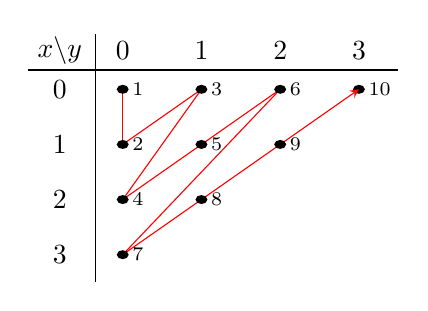
\begin{tikzpicture}[yscale=.7]
			\usetikzlibrary{arrows.meta}
			
			\tikzset{
				myarrow/.style=-stealth
			}
			
			\foreach \x in {0,1,2,3} {
				\node at (.2,-\x-1) {\x};
			}
			\foreach \y in {0,1,2,3} {
				\node at (\y+1,-.3) {\y};
			}
			\draw[red] (1,-1) -- (1,-2);
			\draw[red] (1,-2) -- (2,-1);
			\draw[red] (2,-1) -- (1,-3);
			\draw[red] (1,-3) -- (3,-1);
			\draw[red] (3,-1) -- (1,-4);
			\draw[red] (1,-4) -- (3+.2,-2+.2);
			
			\node at (.2,-.3) {$x\backslash y$};
			\foreach \x in {0,1,2,3} {
				\foreach \y in {0,1,2,3} {
					\ifthenelse{\x<\y \OR \x=\y}{
						\draw[thick,fill] (4-\y,-\x-1) circle (.06);
					}{}
				}
			}
			\draw[myarrow,red] (3+.2,-2+.2) -- (4,-1);
			\node[right] at (1,-1) {\scriptsize 1};
			\node[right] at (1,-2) {\scriptsize 2};
			\node[right] at (2,-1) {\scriptsize 3};
			\node[right] at (1,-3) {\scriptsize 4};
			\node[right] at (2,-2) {\scriptsize 5};
			\node[right] at (3,-1) {\scriptsize 6};
			\node[right] at (1,-4) {\scriptsize 7};
			\node[right] at (2,-3) {\scriptsize 8};
			\node[right] at (3,-2) {\scriptsize 9};
			\node[right] at (4,-1) {\scriptsize 10};
			
			\draw (-.2,-.65) -- (4.5,-.65);
			\draw (.65,0) -- (.65,-4.5);
			
\end{tikzpicture}

	\end{minipage}
\end{center}

Il valore $\langle x,y \rangle$ rappresenta l'incrocio tra la $x$-esima riga e la $y$-esima colonna. Per costruirla:
\begin{enumerate}
	\item $x = 0$
	\item si parte dalla cella $(x,0)$ e si enumerano le celle della diagonale identificata da $(x,0)$ e $(0,x)$
	\item si incrementa $x$ di $1$ e si ripete dal punto precedente
\end{enumerate}

La funzione deve essere: 
\begin{itemize}
	\item iniettiva: non ci possono essere celle con lo stesso numero
	\item suriettiva: ogni numero in $\mathbb{N}^+$ deve comparire
\end{itemize}
Entrambe le proprietà sono soddisfatte, in quanto la numerazione avviene in maniera incrementale, quindi ogni numero prima o poi compare in una cella e di conseguenza ho una coppia che lo genera.\\

\subsubsection{Forma analitica} 
Per la definizione di $\langle x,y \rangle$ si può notare che
$$ \langle x,y \rangle = \langle x + y,0 \rangle + y $$

\begin{center}
	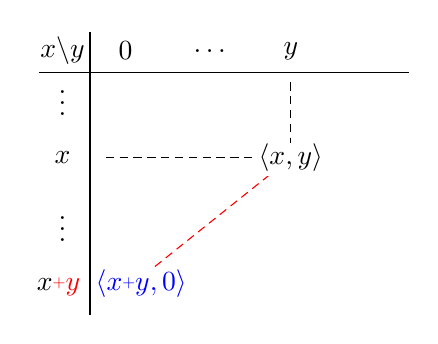
\begin{tikzpicture}[yscale=.8]
		\usetikzlibrary{arrows.meta}
		
		\newcommand{\smallerplus}{\raisebox{.3\height}{\scalebox{.6}{+}}}
		
		\draw[red,densely dashed] (1,-4) -- (3,-2);
		\draw[densely dashed] (.65,-2) -- (3,-2);
		\draw[densely dashed] (3,-1+.2) -- (3,-2);
		
		\node at (.1,-.3) {$x\backslash y$};
		
		\node at (2+1,-.3) {$y$};
		\node at (.9,-.3) {0};
		\node at (1+1,-.3) {$\dots$};
		\node at (.1,-1) {$\vdots$};
		\node at (.1,-1-1) {$x$};
		\node at (.1,-2-1) {$\vdots$};
		\node at (.05,-3-1-.05) {$x{\color{red}\smallerplus y}$};
		\def \offset {.28}
		\draw[white,fill] (3-\offset-.15,-2-\offset) rectangle (3+\offset+.05,-2+\offset-.05);
		\node at (3,-2) {$\langle x,y \rangle$};
		\draw[white,fill] (1-\offset-.15,-4-\offset) rectangle (1+\offset+.05,-4+\offset-.05);
		\node[blue] at (1.1,-4) {$\langle x \smallerplus y, 0 \rangle$};
		
		\draw (-.2,-.65) -- (4.5,-.65);
		\draw (.45,0) -- (.45,-4.5);
\end{tikzpicture}	

\end{center}

Intuitivamente, a partire da $\langle x + y, 0\rangle$ mi basta "salire" seguendo la diagonale fino a $\langle x,y$, ovvero $y$ posti, e per definizione della funzione, $y$ valori più in alto.\\

Il calcolo della funzione coppia si può quindi ridurre al calcolo di $\langle x + y, 0$. Chiamando $x + y = z$, si può notare come ogni cella 
$$ \langle z,0 \rangle = z + \langle z - 1, 0 \rangle $$
E di conseguenza
\begin{align*}
	\langle z,0 \rangle & = z + \langle z - 1, 0 \rangle \\
	& = z + (z-1) + \langle z-2, 0 \rangle \\
	& = z + (z-1) + \dots + 1 + \langle 0,0 \rangle = \\
	& = \sum_{i=1}^{z} i + 1 = \frac{z(z+1)}{2} + 1
\end{align*}

Mettendo insieme le due proprietà viste possiamo ottenere la formula analitica per la funzione coppia: 
$$ \langle x,y \rangle = \langle x + y, 0 \rangle + y = \frac{(x + 1) (x + y + 1)}{2} + y + 1 $$

\subsubsection{Forma analitica di $\sin$ e $\des$} 
Vogliamo fare la stessa cosa per $\sin$ e $\des$, in modo da poter computare l'inversa della funzione coppia, dato $n$. Grazie alle osservazioni precedenti sappiamo che
$$ \begin{array}{r c l}
	\gamma = x + y & \implies & x = \gamma + y \\
	n = y + \langle \gamma , 0 \rangle & \implies & y = n - \langle \gamma , 0 \rangle \\
\end{array} $$

Trovando il valore di $\gamma$ possiamo trovare $x$ e $y$. \\

Notiamo come $\gamma$ sia il più grande valore che, quando calcolato sulla prima colonna ($\langle \gamma, 0 \rangle$) non supera $n$, ovvero
$$ \gamma = \max \{z \in \mathbb{N} | \langle z, 0 \rangle \leq n \} $$
Intuitivamente, si tratta dell'inizio della diagonale che contiene $n$, è "l'inverso" dell'osservazione fatta in precedenza per la quale $ \langle x,y \rangle = \langle x + y,0 \rangle + y $.\\

Risolviamo quindi la disequazione
\begin{align*}
	\langle z, 0 \rangle \leq n & \implies \frac{z(z+1)}{2} + 1 \leq n \\
	& \implies z^2 + z - 2n + 2 \leq 0 \\
	& \implies z_{1,2} = \frac{-1 \pm \sqrt{1 + 8n - 8}}{2} \\
	& \implies \frac{-1 - \sqrt{8n - 7}}{2} \leq z \leq \frac{-1 + \sqrt{8n - 7}}{2} 
\end{align*}

Come valore di $\gamma$ scegliamo
$$ \gamma = \left\lfloor \frac{-1 + \sqrt{8n - 7}}{2} \right\rfloor $$

E con $\gamma$ noto possiamo definire le funzioni $\sin$ e $\des$ come
$$ 
\begin{array}{r c l}
	\des(n) & = & y = n - \langle \gamma, 0 \rangle = n - \frac{\gamma (\gamma + 1)}{2} - 1 \\
	\sin (n) & = & x = \gamma - y
\end{array}
$$

\begin{theor}
	$\mathbb{N} \times \mathbb{N} \sim \mathbb{N}^+$
\end{theor}
\begin{proof}
	La funzione di Cantor è una funzione biettiva tra l'insieme $\mathbb{N} \times \mathbb{N}$ e l'insieme $\mathbb{N}^+$, quindi i due insiemi sono isomorfi.\\
\end{proof}

Possiamo estendere il risultato all'interno dell'insieme $\mathbb{N}$, ovvero:

\begin{theor}
	$\mathbb{N} \times \mathbb{N} \sim \mathbb{N}$
\end{theor}
\begin{proof}
	Definiamo la funzione 
	$$ [,]: \mathbb{N} \times \mathbb{N} \rightarrow \mathbb{N} $$
	tale che
	$$ [x,y] = \langle x,y \rangle - 1$$
	Questa funzione è anch'essa biettiva, quindi i due insiemi sono isomorfi.\\
\end{proof}

Grazie a questo è possibile dimostrare anche che $\mathbb{Q} \sim \mathbb{N}$, infatti i numeri razionali si possono rappresentare come coppie (num, den) e, in generale, tutte le tuple sono isomorfe e $\mathbb{N}$, basta iterare in qualche modo la funzione coppia di Cantor.\\

\subsection{Applicazione alle strutture dati}

I risultati ottenuti fin'ora rendono intuibile come ogni dato possa essere trasformato in un numero, soggetto a trasformazioni matematiche. La dimostrazione \textit{formale} non verrà fatta, anche se verranno fatti esempi di alcune strutture dati che possono essere trasformate in un numero tramite la funzione coppia di Cantor. Ogni struttura dati può essere manipolata e trasformata in una coppia $(x,y)$.\\

Le \textbf{liste} sono le strutture dati più utilizzate nei programmi. In generale non ne è nota la grandezza, di conseguenza è necessario trovare un modo, soprattutto durante l'applicazione di $\sin$ e $\des$, per capire quando abbiamo esaurito gli elementi della lista.\\

Estendiamo la funzione coppia a una lista di interi $x_1, \dots, x_n$:
$$ \langle x_1, \dots, x_n \rangle \rightarrow \langle x_1, \langle x_2 \langle \dots \langle x_n, 0 \rangle \dots \rangle \rangle \rangle $$

Lo $0$ rappresenta il fine lista e non è necessario nel caso in cui il numero di elementi è noto.\\

La decodifica è il processo inverso, partendo dal numero finale si applicano le funzioni $\sin$ e $\des$ ottenendo a ogni iterazione: 
\begin{itemize}
	\item da $\des$ la somma parziale, su cui riapplicare la funzione per ottenere il valore successivo
	\item da $\sin$ il valore presente all'interno della lista
\end{itemize} 
Termina quando il risultato di $\des$ è zero, ovvero l'elemento di fine lista che abbiamo inserito ($x_n$ nel caso di array).
\begin{center}
	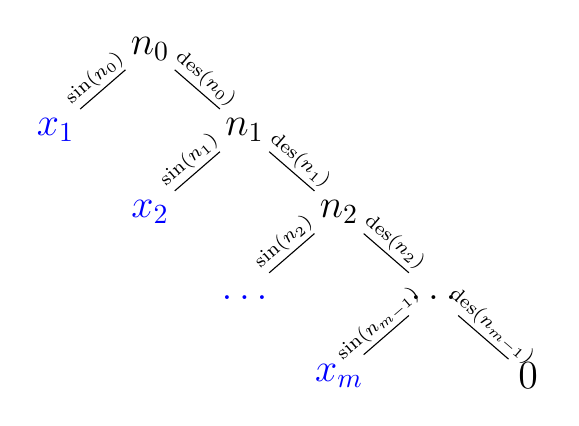
\begin{tikzpicture}[
		level distance=13mm,
		sibling distance=30mm,
		scale=0.8
		]
		\node {\Large$n_0$} 
		child {node[blue] {\Large$x_1$} 
			edge from parent node[xshift=-3,yshift=4,rotate=40.8] {\scriptsize$\sin(n_0)$}
		}
		child {node {\Large$n_1$}
			child {node[blue] {\Large$x_2$}
				edge from parent node[xshift=-3,yshift=4,rotate=40.8] {\scriptsize$\sin(n_1)$}  
			}
			child {node {\Large$n_2$}
				child {node[blue] {\Large$\phantom{n_1}\dots\phantom{n_1}$}
					edge from parent node[xshift=-3,yshift=4,rotate=40.8] {\scriptsize$\sin(n_2)$}  
				}
				child {node {\Large$\phantom{n_1}\dots\phantom{n_1}$}
					child {node[blue] {\Large$x_m$}
						edge from parent node[xshift=-3,yshift=4,rotate=40.8] {\scriptsize$\sin(n_{m-1})$}  
					}
					child {node {\Large$0$} edge from parent 
						node[xshift=3,yshift=4,rotate=-40.8] {\scriptsize$\des(n_{m-1})$}}
					edge from parent node[xshift=3,yshift=4,rotate=-40.8] {\scriptsize$\des(n_2)$}
				}
				edge from parent node[xshift=3,yshift=4,rotate=-40.8] {\scriptsize$\des(n_1)$}
			}
			edge from parent node[xshift=3,yshift=4,rotate=-40.8] {\scriptsize$\des(n_0)$}
		};
\end{tikzpicture}

\end{center}
Se è presente uno 0 all'interno della lista non è un problema in quanto solo $\des$ viene controllato e lo 0 come valore sarà risultato di $\sin$.\\

Quindi è possibile codificare liste e, di conseguenza, \textbf{qualsiasi tipo di dato}, basta convertirlo in una lista di numeri. Per esempio:
\begin{itemize}
	\item una matrice può essere vista come array di array
	\item un grafo può essere rappresentato tramite la sua matrice di adiacenza
	\item i testi sono liste di caratteri
	\item i suoni si possono campionare per ottenere una lista di valori
	\item le immagini sono una "lista" di pixel, ognuno dei quali ha un colore come valore
\end{itemize}

Abbiamo visto come i dati possano essere sostituiti da delle codifiche numeriche; di conseguenza possiamo sostituire tutte le funzioni 
$$ f: \dati \rightarrow \dati \;\; \text{ con funzioni } \;\; f': \mathbb{N} \rightarrow \mathbb{N}_\bot $$

In altre parole, l'universo dei problemi per i quali cerchiamo una soluzione automatica è rappresentabile da $\mathbb{N}_\bot^{\mathbb{N}}$ e di conseguenza $\dati \sim \mathbb{N}$.\\

\section{$\prog \sim \mathbb{N}$}
Adesso lavoriamo sulla parte della relazione che afferma 
$$ F(\C) \sim \prog \sim \mathbb{N} $$

Ovvero, la potenza computazionale (l'insieme dei programmi che un sistema di calcolo $\C$ riesce a calcolare, $F(\C)$) è isomorfa all'insieme di tutti i programmi, a loro volta isomorfi a $\mathbb{N}$.\\

Vogliamo arrivare a ricavare un numero dato un programmo e viceversa. Per farlo servirà vedere l'insieme $\prog$ come l'insieme dei programmi scritti in un certo linguaggio di programmazione.\\

I sistemi analizzati saranno: 
\begin{itemize}
	\item sistema di calcolo $\ram$
	\item sistema di calcolo $\while$
\end{itemize}

Il sistema RAM può apparentemente sembrare "troppo semplice", quindi il sistema WHILE verrà usato per avere un confronto tra le potenze computazionali. Un sistema più sofisticato porta a poter risolvere più problemi? \\

Ci sono due possibili soluzioni: 
\begin{itemize}
	\item $F(\ram \neq F(\while)$: la computabilità \textit{dipende dal sistema usato}
	\item $F(\ram) = F(\while)$: la computabilità è \textit{intrinseca nei problemi} e, di conseguenza, tutti i sistemi sono equivalenti (Tesi di Church-Turing)
\end{itemize}

Il secondo caso è più promettente e, in quel caso, l'obiettivo diventerebbe trovare una \textit{caratterizzazione teorica}, ovvero un "confine" per i problemi calcolabili.\\

\subsection{Sistema di calcolo $\ram$}
Il sistema di calcolo $\ram$ è un sistema semplice che permette di definire rigorosamente: 
\begin{itemize}
	\item $\prog \sim \mathbb{N}$
	\item la \textbf{semantica} dei programmi eseguibili, ovvero $\C(P,\_)$, con $\C = \ram$, ottenendo $\ram (P,\_)$
	\item la \textbf{potenza computazionale}, ovvero calcolare $F(\C)$ con $\C = \ram$, ottenendo $F(\ram)$
\end{itemize}

\subsubsection{Struttura}
Una macchina $\ram$ è formata da un processore e da una memoria teoricamente infinita, divisa in \textbf{celle/registri} contenenti numeri naturali (dati aritmetizzati).\\

Indichiamo i \textbf{registri} con $R_k$, con $k \geq 0$. Tra questi 
\begin{itemize}
	\item $R_0$ contiene l'output
	\item $R_1$ contiene l'input
\end{itemize}

Inoltre è presente un registro $L$, anche detto \textbf{program counter} $PC$ che indica l'indirizzo dell'istruzione successiva.\\

Dato un \textbf{programma} $P$, indichiamo con $|P|$ il numero di istruzioni che il programma contiene.\\

Le \textbf{istruzioni} nel linguaggio RAM sono: 
\begin{itemize}
	\item \textbf{incremento}: $R_k \leftarrow R_k + 1$
	\item \textbf{decremento}: $R_k \leftarrow R_k - 1$
	\item \textbf{salto condizionato}: \texttt{if $R_k = 0$ then goto $m$}, con $m \in \{1, \dots, |P|\}$
\end{itemize}
L'istruzione di decremento è tale che
$$ x - y = \begin{cases}
	x-y & \text{ se } x \geq y\\
	0 & \text{ altrimenti }
\end{cases}$$

\begin{center}
	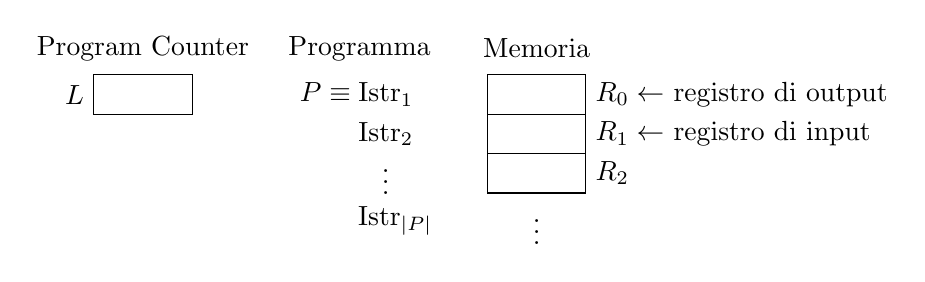
\begin{tikzpicture}
    \node[above] at (.875,.6) {Memoria};

    \draw (.25,0) rectangle (1.5,.5);
    \node[right] at (1.5,.25) {$R_0 \leftarrow$ registro di output};
    \draw (.25,-.5) rectangle (1.5,0);
    \node[right] at (1.5,-.25) {$R_1 \leftarrow$ registro di input};
    \draw (.25,-1) rectangle (1.5,-.5);
    \node[right] at (1.5,-.75) {$R_2$};
    
    \node[below] at (.875,-1) {$\vdots$};

    \def\y{2.25}
    \node[above] at (.875-\y,.55) {Programma};
    \node[] at (.84-\y,.25) {$P\equiv\text{Istr}_1$};
    \node[] at (1.21-\y,-.25) {$\text{Istr}_2$};
    \node[] at (1.21-\y,-.75) {$\vdots$};
    \node[] at (1.33-\y,-1.35) {$\text{Istr}_{|P|}$};

    \def\x{5}
    \node[above] at (.875-\x,.55) {Program Counter};

    \draw (.25-\x,0) rectangle (1.5-\x,.5);
    \node[left] at (1.5-1.25-\x,.25) {$L$};
\end{tikzpicture}

\end{center}

\subsubsection{Esecuzione di un programma RAM}

L'esecuzione di un programma su una macchina RAM segue i passi:
\begin{enumerate}
	\item \textbf{Inizializzazione}:
	\begin{itemize}
		\item viene caricato il programma $P \equiv \text{Istr}_1, \dots \text{Istr}_n$ in memoria
		\item il PC viene posto a 1 per indicare di eseguire la prima istruzione del programma
		\item viene caricato l'input in $R_1$
		\item ogni altro registro è azzerato
	\end{itemize}
	\item \textbf{Esecuzione}: le istruzioni vengono eseguite una dopo l'altra, a ogni iterazione passa da $L$ a $L+1$ (escluse operazioni di salto). Essendo il linguaggio RAM \textit{non strutturato} richiede un PC per sapere l'operazione da eseguire al passo successivo.
	\item \textbf{Terminazione}: per convenzione, si usa $L=0$ per indicare che l'esecuzione del programma è terminata o andata in loop. Nel caso in cui il programma termini, è detto \textbf{segnale di halt} e arresta la macchina
	\item \textbf{Output}: il contenuto di $R_0$, in caso di halt, contiene il risultato dell'esecuzione del programma $P$. Si indica con $\varphi_P(n)$ il contenuto del registro $R_0$ in caso di halt, oppure $\bot$ in caso di loop
	$$ 
	\varphi_P (n) = \begin{cases}
		cont(R_0) & \text{ se halt} \\
		\bot & \text{ se loop}
	\end{cases}
	$$
\end{enumerate}
Con $\varphi_P: \mathbb{N} \rightarrow \mathbb{N}_\bot$ indichiamo la semantica del programma $P$.\\

Con $\C(P,\_)$ indicavamo la semantica di $P$ nel sistema di calcolo $\C$, quindi con $\ram(P,\_) = \varphi_P$ indichiamo la semantica di $P$ nel sistema di calcolo RAM.\\

\subsubsection{Semantica Operazionale}

Per dare una definizione formale della semantica di un programma RAM va specificato il significato di ogni istruzione (\textbf{semantica operazionale}), esplicitando l'effetto che quell'istruzione ha sui registri della macchina.\\

Ogni istruzione fa passare la macchina da uno stato all'altro e la \textbf{semantica operazionale} di un'istruzione è la \textbf{coppia} formata dagli \textbf{stati} della macchina \textbf{prima e dopo l'istruzione}.
$$ \text{STATO}_1 \rightarrow \boxed{\text{Istr}_i} \rightarrow \text{STATO}_2 $$
$$ (\text{STATO}_1,\text{STATO}_2) = \text{semantica operazionale di Istr}_i $$

Uno stato deve descrivere completamente la situazione della macchina in un certo istante. Il programma rimane uguale, quindi l'informazione da salvare è la situazione globale dei registri $R_k$ e il registro $L$.\\

La \textbf{computazione} del programma $P$ è una sequenza di stati $\st_i$, ognuno generato dall'esecuzione di un'istruzione del programma; $P$ induce una sequenza di stati $\st_i$, se questa è formata da un numero infinito di stati, allora il programma è andato in loop; in caso contrario, nel registro $R_0$ si trova il risultato $y$ della computazione di $P$.
$$ 
\varphi_P: \mathbb{N} \rightarrow \mathbb{N}_\bot \tc \varphi_P(n) = \begin{cases}
	y & \text{ se } \exists \st_{fin} \\
	\bot & \text{ altrimenti}
\end{cases}
$$

Per definire come passare da uno stato all'altro, definiamo formalmente: 
\begin{itemize}
	\item \textbf{Stato}: istantanea di tutte le componenti della macchina, è una funzione 
	$$ \st: \{L, R_i\} \rightarrow \mathbb{N} $$
	tale che $\st (R_k)$ restituisce il contenuto del registro $R_k$ quando la macchina si trova nello stato $\st$. Gli stati possibili di una macchina appartengono all'insieme 
	$$ \stati = \{f: \{L, R_i\} \rightarrow \mathbb{N}\} = \mathbb{N}^{\{L,R_i\}} $$
	%Questa rappresentazione permette un numero di registri potenzialmente infinito. Se così non fosse, avremmo tuple per indicare tutti i possibili registri al posto dell'insieme $\{L,R_i\}$
	
	\item \textbf{Stato Finale}: uno stato finale $\st_{fin}$ è un qualsiasi stato $\st$ tale che $\st (L) = 0$
	\item \textbf{Dati}: già dimostrato come $\dati \sim \mathbb{N}$
	\item \textbf{Inizializzazione}: serve una funzione che, preso l'input, restituisca lo stato iniziale della macchina: 
	$$ \text{in}: \mathbb{N} \rightarrow \stati \tc \text{in}(n) = \st_{init}$$
	Lo stato iniziale $\st_{init}$ è tale che 
	$$ 
	\st_{init} (R) = \begin{cases}
		1 & \text{ se } R=L \\
		n & \text{ se } R=R_1 \\
		0 & \text{ altrimenti}
	\end{cases}
	$$
	\item \textbf{Programmi}: $\prog$ è definito come l'insieme dei programmi $\ram$
\end{itemize}

Manca da definire la \textit{parte dinamica} del programma, ovvero l'esecuzione. Per farlo, definiamo la \textbf{funzione di stato prossimo}: 
$$ \delta : \stati \times \prog \rightarrow \stati_\bot $$
tale che 
$$ \delta (\st,P) = \st' $$
dove $\st$ rappresenta lo stato attuale e $\st'$ rappresenta lo stato prossimo dopo l'esecuzione di un'istruzione di $P$.\\

La funzione $\delta (\st, P) = \st'$ è tale che
\begin{itemize}
	\item se $\st(L) = 0$ ho halt, ovvero deve terminare la computazione. Poniamo lo stato come indefinito, ovvero $\st' = \bot$
	\item Se $\st(L)>|P|$ vuol dire che $P$ non contiene istruzioni che bloccano esplicitamente l'esecuzione del programma. Lo stato $\st'$ è tale che 
	$$ 
	\st'(R) = \begin{cases}
		0 & \text{ se } R = L \\
		\st(R_i) \text{ se } R = R_i \forall i
	\end{cases}
	$$
	\item Se $1 \leq \st(L) \leq |P|$ considero l'istruzione $\st(L)$-esima:
	\begin{itemize}
		\item se ho un incremento/decremento sul registro $R_k$ definisco $\st'$ tale che 
		$$ 
		\begin{cases}
			\st'(L) & = \st (L) + 1\\
			\st'(R_k) & = \st (R_k) \pm 1\\
			\st'(R_i) & = \st (R_i) \; \text{ per } \; i \neq k \\
		\end{cases}
		$$
		\item Se ho un \texttt{goto} sul registro $R_k$ che salta all'indirizzo $m$, definisco $\st'$ tale che 
		$$ 
		\st' (L) = \begin{cases}
			m & \text{ se } \st (R_k) = 0 \\
			\st (L) + 1 & \text{ altrimenti}
		\end{cases}
		$$
		$$ \st' (R_i) = \st (R_i) \; \forall i $$
	\end{itemize}
\end{itemize}

L'esecuzione di un programma $P \in \prog$ su input $n \in \mathbb{N}$ genera una sequenza di stati 
$$ \st_0, \st_1, \dots, \st_i, \st_{i+1}, \dots $$
tali che 
$$
\begin{array}{l l c l}
	& \st_0 & = & \text{in}(n) \\
	\forall i & \st_{i+1} & = & \delta (\st_i,P) 
\end{array}
$$
La sequenza è infinita quando $P$ va in loop, mentre se termina raggiunge uno stato $\st_m$ tale che $\st_m (L) = 0$, ovvero ha ricevuto il segnale di halt. \\

La semantica di $P$ è 
$$ 
\varphi_P (n) = \begin{cases}
	y & \text{ se } P \text{ termina in } \st_m, \text{ con } \st_m (L) = 0 \text{ e } \st_m(R_0) = y \\
	\bot & \text{ se } $P$ \text{ va in loop}
\end{cases}
$$

La potenza computazionale del sistema $\ram$ è 
$$ F(\ram) = \left\{f \in \mathbb{N}^{\mathbb{N}}_\bot | \exists P \in \prog | \varphi_P = f \right\} = \left\{\varphi_P | P \in \prog \right\} \subsetneq \mathbb{N}^{\mathbb{N}}_\bot $$
L'insieme è formato da tutte le funzioni $f: \mathbb{N} \rightarrow \mathbb{N}_\bot$ che hanno un programma che le calcola in un sistema $\ram$.\\

\subsection{Aritmetizzazione di un programma}

Per verificare che $\prog \sim \mathbb{N}$ basterebbe trovare una funzione che permetta di codificare i programmi in numeri in modo biunivoco. Data una lista di istruzioni semplici $P \equiv \text{Istr}_1, \dots, \text{Istr}_m$ se questa fosse codificata come una lista di interi potremmo sfruttare la funzione coppia di Cantor per ottenere un numero associato al programma $P$.\\

Quindi vogliamo trovare una funzione $Ar$ che associ a ogni istruzione $I_k$ la sua codifica numerica $c_k$. Se la funzione trovata è anche biunivoca siamo sicuri di poter trovare anche la sua inversa, ovvero la funzione che ci permette di ricavare $I_k$ da $c_k$.\\

Riassumendo, vogliamo trasformare la lista di istruzioni un una lista di numeri su cui successivamente applicare la funzione coppia di Cantor. Vorremmo anche ottenere la lista di istruzioni originale data la codifica.
\begin{center}
	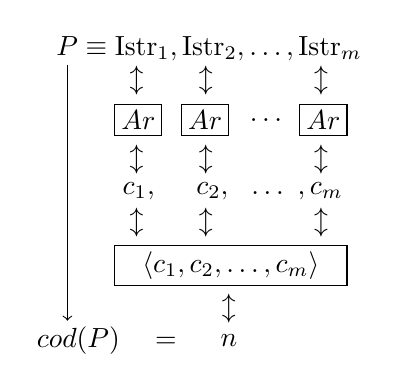
\begin{tikzpicture}
    \node at (0,0)
        {$ P \equiv \text{Istr}_1,\text{Istr}_2,\dots,\text{Istr}_m$};
    \node at (.25,-.4) 
        {$\updownarrow \qquad \updownarrow \qquad \ \ \ \ \ \updownarrow$};
    
    \draw (-1.2,-1.1) rectangle (-.6,-.7) node[midway] {$Ar$};
    \begin{scope}[xshift=.85cm]
        \draw (-1.2,-1.1) rectangle (-.6,-.7) node[midway] {$Ar$};
    \end{scope}
    \begin{scope}[xshift=2.35cm]
        \draw (-1.2,-1.1) rectangle (-.6,-.7) node[midway] {$Ar$};
    \end{scope}
    \node at (.75,-.9) {$\dots$};

    \node at (.25,-1.4) 
        {$\updownarrow \qquad \updownarrow \qquad \ \ \ \ \ \updownarrow$};
    \node at (.3,-1.8) 
        {$c_1,\ \ \ \ c_2, \ \ \dots \  ,c_m$};
    \node at (.25,-2.2) 
        {$\updownarrow \qquad \updownarrow \qquad \ \ \ \ \ \updownarrow$};
    \draw (-1.2,-3) rectangle (1.75,-2.5) node[midway] 
        {$\langle c_1,c_2,\dots,c_m \rangle$};
    \node at (.25,-3.3) {$\updownarrow$};
    \node at (.25,-3.7) {$n$};
    \node at (-1.3,-3.7) {$cod(P) \quad =$};
    \draw [->] (-1.8,-.2) -- (-1.8,-3.45);

\end{tikzpicture}

\end{center} 
L'associazione biunivoca di un numero a una struttura si dice aritmetizzazione o G\"odelizzazione.\\

\subsubsection{Applicazione ai programmi RAM}
Dovendo codificare tre istruzioni nel linguaggio $\ram$, definiamo la funzione $Ar$ tale che
$$ 
Ar(I) = \begin{cases}
	3k & \text{ se } I \equiv R_k \leftarrow R_k + 1 \\
	3k + 1 & \text{ se } I \equiv R_k \leftarrow R_k \dotminus 1 \\
	3k \langle k,m\rangle - 1 & \text{ se } I \equiv \text{ \texttt{if} } R_k = 0 \text{ \texttt{then goto} } m \\
\end{cases}
$$
Per l'inversa, in base al modulo tra $n$ e 3 ottengo una certa istruzione: 
$$
Ar^{-1} (n) = \begin{cases}
	R_{\frac{n}{3}} \leftarrow R_{\frac{n}{3}} + 1 & \text{ se } n \mod 3 = 0 \\
	R_{\frac{n-1}{3}} \leftarrow R_{\frac{n-1}{3}} \dotminus 1 & \text{ se } n \mod 3 = 1 \\
	\text{\texttt{if} } R_{\sin\left(\frac{n+1}{3}\right)} = 0 \text{ \texttt{then goto} } \des\left(\frac{n+1}{3}\right) & \text{ se } n \mod 3 = 2 \\
\end{cases}
$$

Per tornare indietro devo prima invertire la funzione coppia di Cantor e poi invertire la funzione $Ar$.\\
La lunghezza del programma $P$, indicata con $|P|$, si calcola come $len(cod(P))$.\\

Abbiamo quindi dimostrato che $\prog \sim \mathbb{N}$.\\

\subsubsection{Osservazioni}
Avendo $n = cod(P)$ si può scrivere
$$ \varphi_P (t) = \varphi_n (t) $$
Ovvero, la semantica di $P$ è uguale alla semantica della sua codifica. \\

I numeri diventano un \textit{linguaggio di programmazione}.\\

Si può scrivere l'insieme 
$$ F(\ram) = \{\varphi_P: P \in \prog \}$$
come 
$$ F(\ram) = \{\varphi_i\}_{i \in \mathbb{N}} $$
L'insieme, grazie alla dimostrazione di $\prog \sim \mathbb{N}$, è numerabile.\\

Abbiamo dimostrato rigorosamente che 
$$ F(\ram) \sim \mathbb{N} \nsim \mathbb{N}^{\mathbb{N}}_\bot $$
Di conseguenza, anche nel sistema di calcolo $\ram$ esistono funzioni no calcolabili.\\

La $\ram$ è troppo elementare affinché $F(\ram)$ rappresenti formalmente la "classe dei problemi risolubili automaticamente", quindi considerando un sistema di calcolo $\C$ più sofisticato, ma comunque trattabile rigorosamente come il sistema $\ram$, potremmo dare un'idea formale di "ciò che è calcolabile automaticamente".\\

Se riesco a dimostrare che $F(\ram) = F(\C)$ allora cambiare la tecnologia non cambia ciò che è calcolabile, ovvero la calcolabilità è intrinseca ai problemi, quindi la si può caratterizzare matematicamente. \\

\subsection{Sistema di calcolo $\while$}
Introduciamo quindi il sistema di calcolo $\while$ per vedere se riusciamo a "catturare" più o meno funzioni calcolabili dalla macchina $\ram$.

\subsubsection{Struttura}
La macchina $\while$ ha anch'essa, come la macchina $\ram$, una serie di registri, ma al posto di essere \textit{potenzialmente infiniti} sono esattamente 21. Il registro $R_0$ è il \textbf{registro di output}, mentre $R_1$ è il \textbf{registro di input}. Non esiste il Program Counter in quanto il linguaggio è \textbf{strutturato} e ogni istruzione in questo linguaggio va eseguita in ordine.\\

Il linguaggio $\while$ prevede una \textbf{definizione induttiva}: vengono definiti alcuni comandi base e i comandi più complessi sono una concatenazione dei comandi base.\\

\paragraph{Assegnamento:} Comando di base, ne esistono di tre tipi: 
\begin{align*}
	x_k & := 0, \\
	x_k & := x_j + 1 \\
	x_k & := x_j \dotminus 1
\end{align*}
Queste istruzioni sono più complete rispetto alle istruzioni $\ram$, in una sola istruzione possiamo azzerare il valore di una variabile o assegnare a una variabile il valore di un'altra aumentato/diminuito di 1.

\paragraph{While:} Primo comando "induttivo". Si tratta di un comando della forma: 
\begin{center}
	\texttt{while} $x_k \neq 0$ \texttt{do} $C$
\end{center}
Dove $C$ è detto \textbf{corpo} e può essere un assegnamento, un comando while o un comando composto.

\paragraph{Composto:} Altro comando induttivo. Si tratta di un comando nella forma
\begin{center}
	\texttt{begin} $C_1; \dots; C_n$ \texttt{end}
\end{center}
Dove i vari $C_i$ sono, come prima, assegnamenti, comandi while o comandi composti.\\

\paragraph{Programma $\while$:} Un programma $\while$ è un comando composto, e l'insieme di tutti i programmi $\while$ è l'insieme
$$ W-\prog = \{\prog \text{ scritti in linguaggio } \while \} $$

Chiamiamo 
$$ \Psi_W : \mathbb{N} \rightarrow \mathbb{N}_\bot $$
la \textbf{semantica} del programma $W \in W-\prog$.\\

Per dimostrare una proprietà $P$ di un programma $W \in W-\prog$, data la definizione induttiva del linguaggio $\while$, è naturale procedere induttivamente: 
\begin{enumerate}
	\item dimostro $P$ vera sugli assegnamenti 
	\item suppongo $P$ vera sul comando $C$ e la dimostro vera per \texttt{while $x_k \neq 0$ do $C$}
	\item suppongo $P$ vera sui comandi $C_1, \dots, C_n$ e la dimostro vera per \texttt{begin $C_1; \dots; C_n$ end}
\end{enumerate}

\subsubsection{Esecuzione di un programma $\while$}
L'esecuzione di un programma $\while$ $W$ è composta dalle seguenti fasi: 
\begin{enumerate}
	\item \textbf{Inizializzazione}: ogni registro $x_i$ viene posto a $0$, tranne $x_1$, che contiene l'input $n$
	\item \textbf{Esecuzione}: essendo $\while$ un linguaggio con strutture di controllo, non serve un Program Counter, poiché le istruzioni di $W$ vengono eseguite l'una dopo l'altra
	\item \textbf{Terminazione}: l'esecuzione di $W$ può 
	\begin{itemize}
		\item \textit{arrestarsi}: se arriva al termine delle istruzioni
		\item \textit{non arrestarsi}: se entra in un loop
	\end{itemize}
	\item \textbf{Output}: Se il programma va in halt, l'output è contenuto nel registro $x_0$. Possiamo scrivere
	$$ \Psi_W (n) = \begin{cases}
		cont(x_0) & \text{ se halt} \\
		\bot & \text{ se loop}
	\end{cases}$$
\end{enumerate}

\subsubsection{Definizione formale per l'esecuzione}
Come per i programmi $\ram$, serve una definizione formale per la semantica di un programma $\while$, per la quale servono una serie di elementi
\begin{itemize}
	\item \textbf{Stato}: una tupla grande quanto il numero di variabili, dove quindi $\underline{x} = (c_0, \dots, c_{20})$ rappresenta uno stato, con $c_i$ rappresentante il contenuto della variabile $i$
	\item \textbf{$\wstati$}: Insieme di tutti gli stati possibili, contenuto in $\mathbb{N}^{21}$ vista la definizione degli stati 
	\item \textbf{Dati}: già visto che $\dati \sim \mathbb{N}$
	\item \textbf{Inizializzazione}: Lo stato iniziale è descritto dalla funzione 
	$$ w\text{-}in(n) = (0, n, 0, \dots, 0) $$
	\item \textbf{Semantica operazionale}: Vogliamo trovare una funzione che, presi comando da eseguire e stato corrente, restituisce lo stato successivo
\end{itemize}

\paragraph{Funzione stato prossimo:} Soffermandoci sull'ultimo punto, vogliamo trovare la funzione
$$  \llbracket \rrbracket (): \wcom \times \wstati \rightarrow \wstati_\bot $$
Che, dati un comando $C$ del linguaggio $\while$ e lo stato corrente $\underline{x}$, calcoli
$$ \llbracket C \rrbracket (\underline{x}) = \underline{y} $$
con $\underline{y}$ stato prossimo. Quest'ultimo dipende dal comando $C$, ma essendo $C$ induttivo, possiamo provare a dare una definizione induttiva della funzione.\\

Partendo dal passo base, gli \textbf{assegnamenti}:
$$
\llbracket x_k := 0 \rrbracket (\underline{x}) = \underline{y} = \begin{cases}
	x_i & \text{ se } i \neq k \\
	0 & \text{ se } i = k
\end{cases}
$$
$$ 
\llbracket x_k := x_j \pm 1 \rrbracket (\underline{x}) = \underline{y} = \begin{cases}
	x_i & \text{ se } i \neq k \\
	x_j \pm 1 & \text{ se } i = k
\end{cases}
$$

Proseguiamo con il \textbf{passo induttivo}:
\begin{itemize}
	\item \textbf{Comando composto}: vogliamo calcolare
	$$ \llbracket \text{\texttt{begin }} C_1; \dots; C_n \text{\texttt{ end}} \rrbracket (\underline{x}) $$
	Conoscendo ogni $\llbracket C_i \rrbracket$ per ipotesi induttiva, calcoliamo la funzione
	$$ \llbracket C_n \rrbracket \left(\dots \left(\llbracket C_2 \rrbracket \left(\llbracket C_1 \rrbracket (\underline{x})\right)\right) \dots \right) = \left(\llbracket C_n \rrbracket \circ \dots \circ \llbracket C_1 \rrbracket \right) (\underline{x}) $$
	Ovvero, applichiamo in ordine i comandi $C_i$ presenti nel comando composto $C$
	
	\item \textbf{Comando while}: vogliamo calcolare
	$$ \llbracket \text{\texttt{while }} x_k \neq 0 \text{ \texttt{do} } C \rrbracket (\underline{x}) $$
	Conoscendo ogni $\llbracket C_i \rrbracket$ per ipotesi induttiva, calcoliamo la funzione 
	$$ \llbracket C \rrbracket \left(\dots \left(\llbracket C \rrbracket (\underline{x})\right) \dots \right) $$
	Bisogna capire quante volte eseguire il ciclo: dato $\llbracket C \rrbracket^e$ (comando $C$ eseguito $e$ volte) vorremmo trovare il valore di $e$. Questo è il numero minimo di iterazioni che portano in uno stato in cui $x_k = 0$, ovvero il comando \texttt{while} diventa
	$$ \text{\texttt{while} } x_k \neq 0 \text{ \texttt{do} } C = \begin{cases}
		\llbracket C \rrbracket^e (\underline{x}) & \text{ se } e = \mu_t \\
		\bot & \text{ altrimenti}
	\end{cases}$$
	Il valore $e = \mu_t$ è quel numero tale che $\llbracket C \rrbracket^e (\underline{x})$ ha  la $k$-esima componente dello stato uguale a 0
\end{itemize}

Definita la semantica operazionale, manca solo da definire cos'è la \textbf{semantica del programma} $W$ su input $n$. Questa è la funzione 
$$ \Psi_W: \mathbb{N} \rightarrow \mathbb{N}_\bot \; | \; \Psi_W (n) = \text{Proj}\left(0, \llbracket W \rrbracket (w\text{-}in(n))\right)$$

Questo è valido in quanto $W$ programma $\while$ è un programma composto, e abbiamo definito come deve comportarsi la funzione $\llbracket \rrbracket ()$ sui comandi composti.\\

\paragraph{Potenza Computazionale:} La potenza computazionale del sistema di calcolo $\while$ è l'insieme 
$$ F(\while) = \left\{f \in \mathbb{N}^{\mathbb{N}}_\bot | \exists W \in \wprog | f = \Psi_W \right\} = \left\{\Psi_W : W \in \wprog \right\}$$

Ovvero, l'insieme formato da tutte le funzioni che possono essere calcolate con un programma in $\wprog$.\\

\subsection{Confronto tra macchina $\ram$ e $\while$}
Viene naturale confrontare i due sistemi presentati per capire il "più potente", sempre che ce ne sia uno. Le possibilità sono: 
\begin{itemize}
	\item $F(\ram) \subsetneq F(\while)$, data l'estrema semplicità del sistema $\ram$
	\item $F(\ram) \cap F(\while) = \emptyset$, avere insiemi disgiunti significherebbe che il concetto di calcolabile dipende dalla macchina considerata
	\item $F(\while) \subseteq F(\ram)$, che sarebbe sorprendente vista l'apparente maggiore sofisticatezza del sistema $\while$
	\item $F(\while) = F(\ram)$, ovvero il concetto di calcolabile non dipende dalla tecnologia utilizzata ma è intrinseco nei problemi
\end{itemize}

\paragraph{Confronto tra sistemi di calcolo:} Ponendo di avere $\C_1$ e $\C_2$ sistemi di calcolo con programmi in $\cprog{1}$ e $\cprog{2}$ e le relative potenze computazionali
$$ F(\C_1) = \left\{f: \mathbb{N} \rightarrow \mathbb{N}_\bot | \exists P_1 \in \cprog{1} | f = \Psi_{P_1} \right\} = \left\{\Psi_{P_1}: P_1 \in \cprog{1} \right\} $$
$$ F(\C_2) = \left\{f: \mathbb{N} \rightarrow \mathbb{N}_\bot | \exists P_2 \in \cprog{2} | f = \Psi_{P_2} \right\} = \left\{\Psi_{P_2}: P_2 \in \cprog{2} \right\} $$

Mostrare che il primo sistema non è più potente del secondo $F(\C_1) \subseteq F(\C_2)$ vuol dire dimostrare che ogni elemento nel primo insieme deve stare anche nel secondo
$$ \forall f \in F(\C_1) \implies f \in F(C_2) $$

\textit{Espandendo} la definizione di $f \in F(\C)$ la relazione diventa
$$ \forall P_1 \in \cprog{1} | f = \Psi_{P_1} \implies \exists P_2 \in \cprog{2} | f = \Psi_{P_2} $$

Per ogni programma calcolabile nel primo sistema di calcolo ne esiste uno con la stessa semantica nel secondo sistema. Vogliamo trovare un \textbf{compilatore} (o \textbf{traduttore}), ovvero una funzione che trasformi un programma del primo sistema in uno del secondo.\\

\subsubsection{Traduzioni}
Dati $\C_1$ e $\C_2$ due sistemi di calcolo, definiamo \textbf{traduzione} da $\C_1$ a $\C_2$ una funzione
$$ T: \cprog{1} \rightarrow \cprog{2} $$

Con le seguenti proprietà:
\begin{itemize}
	\item \textbf{programmabile}: esiste un modo per programmarla
	\item \textbf{completa}: deve saper tradurre \textit{ogni} programma in $\cprog{1}$ in un programma in $\cprog{2}$
	\item \textbf{corretta}: mantiene la semantica dei programmi di partenza, ovvero
	$$ \forall P \in \cprog{1} \;\; \Psi_P = \varphi_{T(P)}$$
	dove $\Psi$ rappresenta la semantica dei programmi in $\cprog{1}$ e $\varphi$ rappresenta la semantica dei programmi in $\cprog{2}$\\
\end{itemize}


\begin{theor}
	Se esiste $T: \cprog{1} \rightarrow \cprog{2}$ allora $F(\C_1) \subseteq F(\C_2)$
\end{theor}
\begin{proof}
	Se $f \in F(\C_1)$ allora esiste un programma $P_1 \in \cprog{1}$ tale che $\Psi_{P_1} = f$.\\
	
	A questo programma $P_1$ applico $T$, ottenendo $T(P_1) = P_2 \in \cprog{2}$ (per \textit{completezza}) tale che $\varphi_{P_2} = \Psi_{P_1} = f$ (per \textit{correttezza}).\\
	
	Ho trovato un programma $P_2 \in \cprog{2}$ la cui semantica è $f$, allora $F(\C_1) \subseteq F(\C_2)$.\\
\end{proof}

Mostreremo che $F(\while) \subseteq F(\ram)$, ovvero che il sistema $\while$ non è più potente del sistema $\ram$. Costruiremo un compilatore
$$ \comp: \wprog \rightarrow \prog $$
che rispetti le caratteristiche di programmabilità, completezza e correttezza.\\

\subsection{$F(\while) \subseteq F(\ram)$}

Per provare che $F(\while) \subseteq F(\ram)$ vogliamo costruire un compilatore da $\while$ a $\ram$.\\

Per comodità, introduciamo un linguaggio $\ram$ \textit{etichettato}: aggiunge la possibilità di etichettare un'istruzione che indica un punto di salto o di arrivo (stile label assembly). Non altera la potenza espressiva del linguaggio in quanto si tratta di un'aggiunta puramente sintattica: il $\ram$ etichettato si traduce facilmente in $\ram$ puro.\\

Essendo $\wprog$ un insieme definito induttivamente, possiamo definire induttivamente anche il compilatore:
\begin{itemize}
	\item \textbf{Passo base}: come compilare gli assegnamenti
	\item \textbf{Passo induttivo}:
	\begin{enumerate}
		\item Per I.H., assumo di sapere $\comp(C_1), \dots, \comp(C_m)$ e mostro come compilare il comando composto \texttt{begin $C_1; \dots; C:n$ end}
		\item Per I.H., assumo di sapere $\comp(C)$ e mostro come compilare il comando \texttt{while $x_k \neq 0$ do $C$}
	\end{enumerate}
\end{itemize}

Nelle traduzioni andremo a mappare la variabile $\while$ $x_k$ nel registro $\ram$ $R_k$. Questo non crea problemi in quanto stiamo mappando un numero finito di registri in un insieme infinito.\\

Il primo assegnamento che mappiamo è $x_k := 0$
\begin{center}
	\renewcommand{\arraystretch}{1.25}
	\begin{tabular}{l|r l|}
		\cline{2-3}
		$\comp(x_k:=0) =$ & \texttt{LOOP}:& \texttt{IF $R_k = 0$ THEN GOTO EXIT}\\
		&& $R_k\leftarrow R_k \dotminus 1$ \\
		&& \texttt{IF $R_{21} = 0$ THEN GOTO LOOP} \\
		&\texttt{EXIT}:& $R_k \leftarrow R_k \dotminus 1$ \\
		\cline{2-3}
	\end{tabular}\vspace{.15cm}
\end{center}

Questo programma $\ram$ azzera il valore di $R_k$ usando il registro $R_{21}$ per saltare al check della condizione iniziale. Viene utilizzato il registro $R_{21}$ perché, non essendo mappato a nessuna variabile $\while$, sarà sempre nullo dopo la fase di inizializzazione.\\

Gli altri due assegnamenti da mappare sono $x_k:= x_j+1$ e $x_k := x_j \dotminus 1$:
\begin{itemize}
	\item Se $k=j$, la traduzione è banale e l'istruzione $\ram$ è
	$$ \comp(x_k := x_k \pm 1) = R_k \leftarrow R_k \pm 1 $$
	\item Invece se $k \neq j$ la prima idea è quella di "spostare" $x_j$ in $x_k$ e poi fare $\pm 1$ ma non funziona per due ragioni
	\begin{enumerate}
		\item se $R_k \neq 0$ la migrazione (quindi sommare $R_j$ a $R_k$) non genera $R_j$ dentro $R_k$. Si può risolvere azzerando il registro $R_k$ prima della migrazione
		\item $R_j$ dopo il trasferimento è ridotto a 0, ma questo non è il senso dell'istruzione, vorrei solo "\textit{fotocopiarlo}" dentro $R_k$. Questo può essere risolto salvando $R_j$ in un altro registro, azzerare $R_k$, spostare $R_j$ e ripristinare il valore originale di $R_j$
	\end{enumerate}
%	Ricapitolando: 
%	\begin{itemize}
%		\item salviamo $x_j$ in $R_{22}$, registro \textit{sicuro} perché mai coinvolto in altre istruzioni
%		\item azzeriamo $R_k$
%		\item Rigeneriamo $R_j$ e settiamo $R_k$ da $R_{22}$
%		\item $\pm 1$ in $R_k$
%	\end{itemize}
	Quindi possiamo mappare come:
	\begin{center}
		\renewcommand{\arraystretch}{1.25}
		\begin{tabular}{l|r l|l}\cline{2-3}
			$\comp (x_k := x_j \pm 1)$: & \texttt{LOOP}:& \texttt{IF $R_j = 0$ THEN GOTO E1}
			&\multirow{4}{*}{\hspace{-.2cm}
				$\begin{rcases}
					\phantom{}\\
					\phantom{}\\
					\phantom{}\\
					\phantom{}\\
				\end{rcases}$ Salva $R_j$ in $R_{22}$
			} \\
			&& $R_j\leftarrow R_j \dotminus 1$ & \\
			&& $R_{22} \leftarrow R_{22} + 1$ & \\
			&& \texttt{IF $R_{21} = 0$ THEN GOTO LOOP} & \\
			& \texttt{E1:} & \texttt{IF $R_k = 0$ THEN GOTO E2} &\multirow{3}{*}{\hspace{-.2cm}
				$\begin{rcases}
					\phantom{}\\
					\phantom{}\\
					\phantom{}\\
				\end{rcases}$ Azzera $R_k$
				}\\
			&& $R_k \leftarrow R_k \dotminus 1$ & \\
			&& \texttt{IF $R_{21} = 0$ THEN GOTO EXIT 1} & \\
			& \texttt{E2} & \texttt{IF $R_{22} = 0$ THEN GOTO E3} & \multirow{4}{*}{\hspace{-.2cm} 
			$\begin{rcases}
				\phantom{}\\
				\phantom{}\\
				\phantom{}\\
				\phantom{}\\
				\phantom{}\\
			\end{rcases}$ Rigenera $R_j$ e $R_k$ da $R_{22}$
			} \\
			&& $R_k \leftarrow R_k + 1$ & \\
			&& $R_j \leftarrow R_j + 1$ & \\
			&& $R_{22} \leftarrow R_{22} \dotminus 1$ & \\
			&& \texttt{IF $R_{21} = 0$ THEN GOTO E2} & \\ 
			& \texttt{E3:} & $R_k \leftarrow R_k \pm 1$ & \\
			\cline{2-3} 
		\end{tabular}\vspace{.5cm}
	\end{center}
\end{itemize}

Per I.H. sappiamo come compilare $C_1, \dots C_m$. Possiamo calcolare la compilazione del comando composto come
\begin{center}
	\begin{tabular}{r |l|}
		\cline{2-2}
		$\comp($\texttt{begin $C_1; \dots; C_n$ end$)$} = & $\comp (C_1)$ \\
		& $\dots$ \\
		& $\comp(C_m)$ \\
		\cline{2-2}
	\end{tabular}
\end{center}

Per I.H. sappiamo come compilare $C$. Possiamo calcolare la compilazione del comando \texttt{while} come
\begin{center}
	\begin{tabular}{l |r l|}
		\cline{2-3} 
		$\comp(\text{\texttt{while }} x_k \neq 0 \texttt{ do } C) = $ & \texttt{LOOP:} & \texttt{IF $R_k = 0$ THEN GOTO EXIT} \\
		&& $\comp(C)$ \\
		&& \texttt{IF $R_{21} = 0$ THEN GOTO LOOP} \\
		& \texttt{EXIT:} & $R_k \leftarrow R_k \dotminus 1$ \\
		\cline{2-3}
	\end{tabular}
\end{center}

La funzione
$$ \comp: \wprog \rightarrow \prog $$
appena costruita soddisfa le tre proprietà desiderate in quanto:
\begin{itemize}
	\item Programmabile
	\item Compila sempre 
	\item Mantiene la semantica
\end{itemize}

Di conseguenza
$$ F(\while) \subseteq F (\ram) $$

\subsection{$F(\ram) \subseteq F(\while)$}

Abbiamo mostrato che una macchina $\while$ non è più potente di una macchina $\ram$, ora vogliamo fare l'inverso. Per farlo si userà il concetto di interprete.\\

\subsubsection{Interprete in $\while$ per $\ram$}

Introduciamo il concetto di \textbf{interprete}. Chiamiamo $I_W$ l'interprete scritto in linguaggio $\while$ per programmi scritti in linguaggio $\ram$.\\

$I_W$ prende in input un programma $P \in \prog$ e un dato $x \in \mathbb{N}$ e restituisce "\textit{l'esecuzione}" di $P$ sull'input $x$. Più formalmente, restituisce la semantica di $P$ su $x$, quindi $\varphi_P (x)$.

\begin{center}
	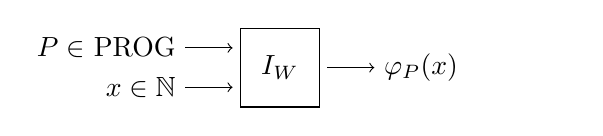
\begin{tikzpicture}
	
	\draw[->] (2.3,1.75) node[left]{$P\in\ $PROG} -- (2.9,1.75);
	\draw[->] (2.3,1.25) node[left]{$x\in \mathbb{N}$} -- (2.9,1.25);
	\draw (3,2) rectangle (4,1);
	\node at (3.5,1.5) {$I_W$};
	\draw[->] (4.1,1.5) -- (4.7,1.5)
	node [right] {$\varphi_P(x)$};
	\node[right] at (4.7,1.5) {$\phantom{\varphi_n(x)=\varphi_P(x)}$};
	
\end{tikzpicture}
\end{center}

Notiamo come l'interprete non crei dei prodotti intermedi, ma si limita a eseguire $P$ sull'input $x$.\\

Due problemi principali: 
\begin{enumerate}
	\item Il primo riguarda il tipo di input della macchina $\while$ in quanto questa non sa leggere il programma $P$ (listato di istruzioni $\ram$), sa leggere solo numeri. Dobbiamo modificare $I_W$ in modo che non passi più $P$ ma la sua codifica $cod(P) = n \in \mathbb{N}$. Questo restituisce la semantica del programma codificato con $n$, che è $P$, quindi $\varphi_n (x) ) \varphi_P (x)$
	\item Il secondo problema riguarda la quantità di dati in input alla macchina $\while$: questa legge l'input da un singolo registro, mentre qui ne stiamo passando due. Bisogna modificare $I_W$, condensando l'input tramite la funzione coppia di Cantor, che diventa $\langle x,n \rangle$
\end{enumerate}
Quindi
\begin{center}
	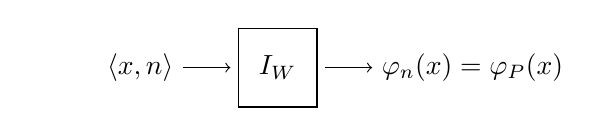
\begin{tikzpicture}
	
	\draw[->] (2.3,1.5) node[left]{$\langle x,n \rangle$} -- (2.9,1.5);
	\node[left] at (2.3,1.5) {$\phantom{cod(P)=n}$};
	\draw (3,2) rectangle (4,1);
	\node at (3.5,1.5) {$I_W$};
	\draw[->] (4.1,1.5) -- (4.7,1.5)
	node [right] {$\varphi_n(x)=\varphi_P(x)$};
	
\end{tikzpicture}
\end{center}

La semantica di $I_W$ diventa
$$ \forall x,n \in \mathbb{N} \;\;\;\; \Psi_{I_W} \left(\langle x,n \rangle \right) = \varphi_n (x) = \varphi_P (x) $$

Similmente a prima, useremo per comodità il linguaggio \textbf{macro-$\while$}, che include alcune macro comode nella scrittura di $I_W$. Viene modificata solo la sintassi e di conseguenza non la potenza del linguaggio.\\

Le \textbf{macro} utilizzate sono: 
\begin{itemize}
	\item $x_k := x_j + x_s$
	\item $x_k := \langle x_j, x_s \rangle$
	\item $x_k := \langle x_1, \dots, x_n \rangle$
	\item $x_k := \proj(x_j, x_s)$, proiezione, estrae l'elemento $x_j$-esimo dalla lista codificata in $x_s$
	\item $x_k := \incr (x_j, x_s)$, incremento, codifica la lista $x_s$ con l'elemento in posizione $x_j$-esima aumentato di 1
	\item $x_k := \decr(x_j, x_s)$, decremento, codifica la lista $x_s$ con l'elemento in posizione $x_j$-esima diminuito di 1
	\item $x_k := \sin (x_j)$
	\item $x_k := \des (x_j)$
	\item Costrutto \texttt{If} \dots \texttt{then} \dots \texttt{else}
\end{itemize}

\subsubsection{Stato della macchina $\ram$ nell'interprete}

Risolto il problema dell'input di un interprete scritto in linguaggio $\while$ per i programmi $\ram$, ora vogliamo scrivere questo interprete. In sintesi, l'interprete esegue una dopo l'altra le istruzioni $\ram$ del programma $P$ e restituisce il risultato $\varphi_P (x)$ (da notare che restituisce il risultato, non un eseguibile).\\

L'interprete ricostruisce virtualmente tutto ciò che gli serve per gestire il programma. Nel caso di $I_W$ deve ricostruire l'ambiente di una macchina $\ram$. Quello che faremo sarà ricreare il programma $P$, il Program Counter $L$ e i registri $R_0, R_1, \dots$, dentro le variabili messe a disposizione dalla macchina $\while$.\\

Primo problema: i programmi $\ram$ possono utilizzare infiniti registri, mentre i programmi $\while$ ne hanno solo 21. \textit{Ma $P$ usa veramente un numero infinito di registri?}

In realtà no; se $cod(P) = n$ allora $P$ non userà mai registri $R_j$ con $j > n$. Il programma $P$ userà sempre un numero finito di registri il cui contenuto può essere racchiuso in una lista $a_0, \dots, a_n$. La soluzione consiste nel raggruppare tutti i valori dei registri tramite Cantor $\langle a_0, \dots, a_n \rangle$ e salvarne la codifica in un unica variabile. Useremo due registri in più per comodità (possono essere utili, you never know).\\

L'interprete $I_W$ salva lo stato della macchina $\ram$ nel seguente modo (con $I_W (\langle x,n\rangle) = \varphi_n (x)$)
\begin{itemize}
	\item $x_0 \leftarrow \langle R_0, \dots, R_{n+2} \rangle$: stato della memoria della macchina $\ram$
	\item $x_1 \leftarrow L$: Program Counter
	\item $x_2 \leftarrow x$: dato su cui lavora $P$
	\item $x_3 \leftarrow n$: "listato" del programma $P$
	\item $x_4$: codice dell'istruzione da eseguire, prelevata da $x_3$ grazie a $x_1$
\end{itemize}

%P39


    % !TeX spellcheck = it_IT
% !TeX root = ../it.tex

\chapter{Teoria della Complessità}

Dato un problema $P$, fino a ora la domanda è stata "\textit{esiste un programma per la sua soluzione automatica?}" E tramite questa domanda si può indagare la teoria della calcolabilità, il cui soggetto di studio è l'esistenza (o meno) di un programma per un dato problema.

La prossima sezione riguarda la \textbf{teoria della complessità} in cui l'investigazione segue la domanda "\textit{come funzionano i programmi per $P$?}".

Per rispondere a questa domanda, vogliamo sapere quante \textbf{risorse computazionali} vengono utilizzate durante la sua esecuzione. Vediamo altre domande a cui la teoria della complessità cerca di rispondere
\begin{itemize}
	\item dato un programma per il problema $P$, quanto tempo impiega nella sua soluzione? Quanto spazio di memoria occupa? 
	\item dato un problema $P$, qual è il minimo tempo impiegato dai programmi per $P$? Quanto spazio in memoria al minimo posso occupare per programmi per $P$? 
	\item in che senso possiamo dire che un programma è \textbf{efficiente} in termini di tempo e/o spazio? 
	\item quali problemi possono essere efficientemente risolti per via automatica?
\end{itemize}

\section{Teoria dei linguaggi formali}

Alcune definizioni:
\begin{itemize}
	\item Un \textbf{alfabeto} è un insieme finito di simboli $\Sigma = \{\sigma_1, \dots, \sigma_k\}$
	\item Un \textbf{alfabeto binario} è un qualsiasi alfabeto composto da due soli simboli
	\item Una \textbf{stringa} su $\Sigma$ è una sequenza di simboli appartenenti a $\Sigma$ nella forma $x = x_1 \cdots x_n$, con $x_i \in \Sigma$
	\item La \textbf{lunghezza} di una stringa $x$ indica il numero di simboli che la costituiscono e si indica con $|x|$
	\item La \textbf{stringa nulla} è una stringa particolare, indicata con $\epsilon$, è tale che $|\epsilon| = 0$
	\item Con $\Sigma^\ast$ si indica l'insieme delle stringhe che si possono costruire sull'alfabeto $\Sigma$ (chiusura di Kleene), compresa la stringa nulla. L'insieme delle stringhe formate da almeno un carattere è $\Sigma^+ = \Sigma^\ast \setminus \{\epsilon\}$
	\item Un \textbf{linguaggio} $L$ su un alfabeto $\Sigma$ è un sottoinsieme $L \subseteq \Sigma^\ast$, che può essere finito o infinito
\end{itemize}

\section{Macchina di Turing Deterministica (DTM)}
Il punto di partenza dello studio della teoria della complessità e la definizione rigorosa delle risorse di calcolo e di come possono essere misurate.

Il modello di calcolo considerato è quello della \textbf{Macchina di Turing}, ideata da Alan Turing nel 1936. Si tratta di un modello teorico di calcolatore che consente di definire rigorosamente: 
\begin{itemize}
	\item i passi di computazione e la computazione stessa
	\item tempo e spazio di calcolo dei programmi
\end{itemize}

\subsection{Struttura}
Una \textbf{Macchina di Turing deterministica} è un dispositivo hardware fornito di: 
\begin{itemize}
	\item \textbf{nastro di lettura/scrittura}: un nastro infinito formato da celle, ognuna delle quali ha un proprio indice/indirizzo e può contenere un simbolo. Questo nastro viene usato come contenitore per l'input, ma anche come memoria durante l'esecuzione
	\item \textbf{testina di lettura e scrittura two-way}: dispositivo che permette di leggere e scrivere dei simboli sul nastro a ogni passo
	\item \textbf{controllo a stati finiti}: automa a stati finiti $Q = \{Q_0, \dots, Q_n\}$ che permette di far evolvere la computazione
\end{itemize}

Un passo di calcolo è una \textbf{mossa} che, dato lo stato corrente e il simbolo letto dalla testina, porta la DTM in un nuovo stato, scrivendo eventualmente un simbolo sul nastro e spostando eventualmente la testine. I risultati della mossa, quindi il nuovo stato, il simbolo da scrivere e il movimento della testina, vengono calcolati tramite una \textbf{funzione di transizione}, basata sui due input dati.

\subsubsection{Definizione Informale}

Il funzionamento di una DTM $M$ su input $x \in \Sigma^\ast$ passa per due fasi:
\begin{enumerate}
	\item \textbf{Inizializzazione}:
	\begin{itemize}
		\item La stringa $x$ viene posta, simbolo dopo simbolo, nelle celle del nastro dalla cella 1 fino alla cella $|x|$. Le celle dopo quelle che contengono $x$ contengono il simbolo \textit{blank}
		\item La testina si posizione sulla prima cella
		\item Il controllo a stati finiti è posto nello stato iniziale
	\end{itemize}
	\item \textbf{Computazione}:
	\begin{itemize}
		\item Sequenza di mosse dettata dalla funzione di transizione
	\end{itemize}
\end{enumerate}

La computazione può andare in loop o arrestarsi se raggiunge una situazione in cui non è definita nessuna mossa per lo stato attuale. Si dice che $M$ accetta $x \in \Sigma^\ast$ se $M$ si arresta in uno stato tra quelli finali/accettanti, altrimenti la rifiuta.

Definiamo $L_M = \{x \in \Sigma^\ast \mid M \text{ accetta } x \}$ il \textbf{linguaggio accettato} da $M$.

\subsubsection{Definizione Formale}
Una DTM è una sestupla $M = \left(Q, \Sigma, \Gamma, \delta, q_0, F\right)$, con:
\begin{itemize}
	\item $Q$: insieme finito di \textbf{stati} assumibili dal controllo a stati finiti
	\item $q_0 \in Q$: \textbf{stato iniziale} da cui partono le computazioni di $M$
	\item $F \subseteq Q$: insieme degli \textbf{stati finali/accettanti} dove $M$ si arresta accettando l'input
	\item $\Sigma$: \textbf{alfabeto di input} su cui sono definite le stringhe di input
	\item $\Gamma$: \textbf{alfabeto di lavoro} che contiene i simboli che possono essere letti/scritti dal/sul nastro. Vale $\Sigma \subset \Gamma$ perché $\Gamma$ contiene il simbolo \textit{blank}
	\item $\delta: Q \times \Gamma \rightarrow Q \times (\Gamma \setminus \{blank\}) \times \{-1, 0, 1\}$: \textbf{funzione di transizione} che definisce le mosse. Si tratta di una funzione parziale: quando non è definita la macchina si arresta. Inoltre, $M$ non può scrivere il simbolo \textit{blank}, lo può solo leggere
\end{itemize}

Analizziamo nel dettaglio lo sviluppo di una DTM $M$ su input $x \in \Gamma^\ast$, visto solo informalmente: 
\begin{enumerate}
	\item \textbf{Inizializzazione}: 
	\begin{itemize}
		\item il nastro contiene la stringa $x = x_1 \cdots x_n$
		\item la testina è posizionata sul carattere $x_1$
		\item il controllo a stati finiti parte dallo stato $q_0$
	\end{itemize}
	\item \textbf{Computazione}: sequenza di mosse definite dalla funzione di transizione $\delta$ che manda, a ogni passo, da $(q_i, \gamma_i)$ a $(q_{i+1}, \gamma_{i+1}, \{-1, 0, +1\})$
\end{enumerate}

Se $\delta(q, \gamma) = \bot$, la macchina $M$ si \textit{arresta}. Quando la testina rimbalza tra due celle o rimane fissa in una sola, si verifica un \textit{loop}. La macchina $M$ accetta $x \in \Sigma^\ast$ se e solo se la computazione si arresta in uno stato $q \in F$. \lcomment{Guarda foto se vuoi Slide 18:9} Come prima, $L_M = \{x \in \Sigma^\ast \mid M \text{ accetta } x\}$ è il \textbf{linguaggio accettato} da $M$.

Queste macchine sono molto simili agli automi a stati finiti, seppur con alcune differenze: 
\begin{itemize}
	\item le FSM di default non possono tornare indietro, non sono two-way, ma questa differenza non aumenta la potenza computazionale, serve solo per avere automi più succinti
	\item le FSM hanno il nastro a sola lettura, mentre le DTM possono alterare il nastro a disposizione
\end{itemize}

\subsubsection{Configurazione di una DTM}

Proviamo, similmente a come fatto per le macchine $\ram$, a dare l'idea di \textbf{configurazione} delle DTM; possiamo vederla come una foto che descrive completamente la macchina $M$ in un certo istante, in questo modo possiamo descrivere la computazione come usa serie di configurazioni/foto.

Le cose da ricordare sono: 
\begin{itemize}
	\item in che stato si trova la macchina
	\item in che posizione si trova la testina
	\item il contenuto non-blank del nastro
\end{itemize}

Definiamo quindi $C = (q,k,w)$ una configurazione con
\begin{itemize}
	\item $q$: stato del controllo a stati finiti
	\item $k \in \N^+$: posizione della testina nel nastro
	\item $w \in \Gamma^+$: contenuto non-blank del nastro
\end{itemize}

All'inizio della computazione si ha la \textbf{configurazione iniziale} $C_0 = (q_0, 1, x)$. Una configurazione $C$ si dice \textbf{accettante} se $C = (q \in F, k, w)$, si dice invece \textbf{d'arresto} se $C = (q, k, w)$, con $\delta (q,w_{k}) = \bot$.

\subsubsection{Definizione di computazione tramite configurazioni}

La computazione di $M$ su $x \in \Sigma^\ast$ è la sequenza
$$ C_0 \xrightarrow{\delta} C_1 \xrightarrow{\delta} \dots \xrightarrow{\delta} C_i \xrightarrow{\delta} C_{i+1} \xrightarrow{\delta} \dots $$
dove $\forall i \geq 0$ vale che da $C_i$ si passa a $C_{i+1}$ grazie alla funzione $\delta$.

La macchina $M$ accetta $x \in \Sigma^\ast$ se e solo se $C_0 \xrightarrow{\ast}C_f$, con $C_f$ configurazione d'arresto e accettante. Il linguaggio accettato da $M$ ha la stessa definizione data prima.

\subsection{Altre versioni delle macchine di Turing}
\subsubsection{Versioni alternative}

Il fatto che la macchina sia \textit{deterministica} implica che, data una configurazione $C_i$, quella successiva è univocamente determinata dalla funzione $\delta$. Quindi, data una configurazione $C_i$, esiste una sola configurazione $C_{i+1}$ successiva, a meno di arresti. \lcomment{Guarda foto se vuoi 18:11}

Nelle \textbf{Macchine di Turing Non Deterministiche (NDTM)}, una configurazione $C_i$ può ammettere più configurazioni successive.

Nelle \textbf{Macchine di Turing Probabilistiche PTM}, data una configurazione $C_i$, possono esistere più configurazioni nelle quali si può entrare, ognuna associata a una probabilità $p_i \in [0,1]$.

Infine, nelle \textbf{Macchine di Turing Quantistiche QTM}, data una configurazione $C_i$, esistono una serie di configurazioni successive nelle quali possiamo entrare osservando le ampiezze delle transizioni $\alpha_i$. Queste ampiezze sono numeri complessi in $\mathbb{C}$ tali che
\begin{itemize}
	\item $|\alpha_i| \leq 1$
	\item hanno probabilità $|\alpha_i|^2$
	\item le probabilità sommano a 1
\end{itemize}

\subsubsection{Versione semplificata}
Esibire, progettare e comprendere una DTM potrebbe risultare difficile, anche per casi semplici. Solitamente, nel descrivere una DTM viene utilizzato uno \textit{pseudocodice} che ne chiarisce la dinamica.

Esistono una serie di teoremi che dimostrano che qualsiasi frammento di programma strutturato può essere tradotto in una DTM formale e viceversa.

\subsubsection{Esempio: parità}
Problema: 
\begin{itemize}
	\item Nome: parità
	\item Istanza: $x \in \N$
	\item Domanda: $x$ è pari?
\end{itemize}

Come codifica utilizziamo quella binaria, ovvero
$$ cod: \N \rightarrow \{0,1\}^\ast $$
Di conseguenza, il linguaggio da riconoscere è 
$$ L_{\text{pari}} = \left\{x \in \{0,1\}^\ast \mid x_1 = 1 \wedge x_{|x|} = 0 \right\} \cup \{0\} $$
Risolvere il problema \textit{parità} significa trovare una DTM $M$ che rappresenta un algoritmo deterministico che riconosce $L_{\text{pari}}$.

Ricordando che $M = \left(Q, \Sigma, \Gamma, \delta, q_0, F\right)$, la seguente macchina riconosce $L_{\text{pari}}$:
\begin{itemize}
	\item $Q = \{p, z_1, \mu, z, r\}$ insieme degli stati
	\item $\Sigma = \{0,1\}$ alfabeto 
	\item $\Gamma = \{0,1, blank\}$ alfabeto di lavoro
	\item $q_0 = p$ stato iniziale
	\item $F = \{z_1, z\}$ insieme degli stati finali
	\item $\delta : Q \times \Gamma \rightarrow Q \times \Sigma \times \{-1, 0, 1\}$ funzione di transizione così definita
	\begin{center}
		\renewcommand{\arraystretch}{1.5}
		\begin{tabular}{| C{40000cm} | C{40000cm} | C{40000cm} | C{40000cm} |}
			\hline
			$\delta$ & \textit{blank} & 0 & 1 \\
			\hline
			$p$ & $\bot$ & $(z_1, 0, +1)$ & $(\mu, 1, +1)$ \\
			\hline
			$z_1$ & $\bot$ & $(r, 0, +1)$ & $(\mu, 1, +1)$ \\
			\hline
			$\mu$ & $\bot$ & $(z, 0, +1)$ & $(\mu, 1, +1)$ \\
			\hline
			$z$ & $\bot$ & $(z, 0, +1)$ & $(\mu, 1, +1)$ \\
			\hline
			$r$ & $\bot$ & $\bot$ & $\bot$ \\
			\hline
		\end{tabular}
	\end{center}
\end{itemize}

Si può notare come, anche per un problema così semplice, si ha una funzione di transizione abbastanza complessa. Andiamo quindi a utilizzare uno pseudocodice:
\begin{center}
	\begin{minipage}{.7\textwidth}
		\begin{tcolorbox}[
			colback=white,
			sharp corners,
			boxrule=.3mm,
			left=20pt,
			top=0pt,
			bottom=0pt,
			title=Parità$(n)$,
			colbacktitle=white,
			coltitle=black
			]
			\LinesNumbered
			\begin{algorithm}[H]
				\setstretch{1.2}
				\SetArgSty{relax}
				\SetAlgoNoEnd
				\SetKwProg{if}{if}{}{}
				\SetKwProg{els}{else}{}{}
				\SetKwProg{Do}{do}{}{}
				\SetKwProg{While}{while}{}{}
				\SetKwSty{texttt}
				$i:=1$ \\
				$f:=false$ \\
				\Switch{$x[i]$}{
					\Case{0}{
						$i++$ \\
						$f:= (x[i] == blank)$ \\
						break\\
					}
					\Case{1}{
						\Do{}{
							$f:= (x[i] == 0)$ \\
							$i++$ \\
						}
						\While{$(x[i] \neq blank)$}{}
					}
				}
				\Return{$f$}
			\end{algorithm}
		\end{tcolorbox}
	\end{minipage}
\end{center}

Alla fine dell'esecuzione avremo: 
\begin{itemize}
	\item \textit{True} se $x \in L_{\text{pari}}$
	\item \textit{False} se $x \notin L_{\text{pari}}$
\end{itemize}

\section{Funzionalità di una DTM}

\subsection{Insiemi riconosciuti}

La principale funzionalità di una DTM è \textbf{riconoscere linguaggi}. Un linguaggio $L \subseteq \Sigma^\ast$ è \textbf{riconoscibile} da una DTM se e solo se esiste una DTM $M$ tale che $L = L_M$.

Grazie alla possibilità di riconoscere linguaggi, una DTM può riconoscere anche insiemi: dato $A \subseteq \N$, \textit{come lo riconosco con una DTM?} La prima idea è quella di codificare ogni elemento $a \in A$ in un elemento di $\Sigma^\ast$, per poter passare dal riconoscimento di un insieme al riconoscimento di un linguaggio.
$$
\renewcommand{\arraystretch}{1.8}
A \rightsquigarrow \begin{array}{|c|}
	\hline
	cod \\
	\hline
\end{array}
\rightsquigarrow L_A = \{cod(a): a \in A\}
$$

Un insieme $A$ è riconoscibile da una DTM se e solo se esiste una DTM $M$ tale che $L_A = L_M$.

Quando si fa riconoscere un insieme $A$ a una DTM $M$, possono risultare due situazioni, in funzione dell'input (codificato):
\begin{enumerate}
	\item se l'input appartiene ad $A$, allora $M$ si arresta
	\item se l'input \textit{non} appartiene ad $A$, allora $M$ può 
	\begin{itemize}
		\item arrestarsi rifiutando l'input, ovvero finisce in uno stato $q \notin F$, ma allora $A$ è ricorsivo
		\item andare in loop, ma allora $A$ è ricorsivamente numerabile \\
	\end{itemize}
\end{enumerate}

\begin{theor}
	La classe degli insiemi riconosciuti da una DTM coincide con la classe degli insiemi ricorsivamente numerabili.
\end{theor}

Un algoritmo deterministico per il riconoscimento di un insieme $A \subseteq \N$ è una DTM $M$ tale che $L_A = L_M$ e tale che $M$ si arresta su ogni input.\\

\begin{theor}
	La classe degli insiemi riconosciuti da algoritmi deterministici coincide con la classe degli insiemi ricorsivi.
  \end{theor}

% FINITO QUI DEVI FARE LEZIONE 19

\subsection{Problemi di decisione}

Una seconda funzionalità delle DTM è quella di risolvere \textbf{problemi di decisione}. Dato un problema $\Pi$, con istanza $x \in D$ e domanda $p(x)$, andiamo a codificare gli elementi di $D$ in elementi di $\Sigma^\ast$, ottenendo $L_\Pi = \{cod(x) \mid x \in D \wedge p(x) \}$ \textbf{insieme delle istanze (codificate) a risposta positiva di $\Pi$}.

La DTM risolve $\Pi$ se e solo se $M$ è un algoritmo deterministico per $L_\Pi$, ovvero: 
\begin{itemize}
	\item se vale $p(x)$, allora $M$ accetta la codifica di $x$
	\item se non vale $p(x)$, allora $M$ si arresta senza accettare
\end{itemize}

\subsection{Calcolo di funzioni}

Oltre a ciò che è già stato detto, le DTM sono anche in grado di \textbf{calcolare funzioni}. Si tratta di un risultato molto importante, in quanto sappiamo che calcolare funzioni significa risolvere problemi del tutto generali, quindi non solo di decisione.

Data una funzione $f: \Sigma^\ast \rightarrow \Gamma^\ast$, la DTM $M$ calcola $f$ se e solo se
\begin{itemize}
	\item se $f(x) \downarrow$ allora $M$ su input $x$ termina con $f(x)$ sul nastro
	\item se $f(x) \uparrow$ allora $M$ su input $x$ va in loop
\end{itemize}
A tutti gli effetti le DTM sono \textit{sistemi di programmazione}.

\subsection{Potenza computazionale}

Si può dimostrare che le DTM calcolano tutte e sole le funzioni ricorsive parziali. Possiamo riscrivere la tesi di Church-Turing come: 
\begin{center}
	\textit{Una funzione è intuitivamente calcolabile se e solo se è calcolata da una DTM}
\end{center}

Inoltre, è possibile dimostrare che le DTM sono SPA, semplicemente mostrando che valgono i tre assiomi di Rogers: 
\begin{enumerate}
	\item le DTM calcolano tutte e sole le funzioni ricorsive parziali 
	\item esiste una DTM universale che simula tutte le altre
	\item vale il teorema $S^m_n$
\end{enumerate}

\section{Simboli di Landau}

Nella teoria delle complessità la domanda è \textit{"quanto costa questo programma?"} Per capire il costo di un dato programma verranno valutate delle funzioni nella forma $f(n)$, dove $n$ indica la grandezza dell'input della DTM. Nel fare il confronto tra due algoritmi per uno stesso problema, bisogna tenere in considerazione che a fare la differenza (in termini di prestazioni) sono gli input di dimensione \textit{ragionevolmente grande}, dove con questa espressione intendiamo una dimensione significativa nel contesto d'applicazione del problema.

Per esempio, siano $t_1$ e $t_2$ due funzioni tali che
$$ t_1 (n) = 2n \quad \mid \quad t_2 (n) = \frac{1}{100} n^2 + \frac{1}{2}n + 1 $$

Quale delle due è migliore? \textit{Dipende}, per $n$ abbastanza piccoli allora $t_2$ è migliore, mentre per $n$ sufficientemente grandi allora è migliore $t_1$.

Date due funzioni, non vanno valutate per valori precisi di $n$, ma ne va valutato il loro \textbf{andamento asintotico}, ovvero quando $n$ tende a $+ \infty$.

\subsection{Simboli di Landau principali}

I \textbf{simboli di Landau} sono utili per stabilire degli \textbf{ordini di grandezza} tra le funzioni, in modo da poterle paragonare. I più utilizzati sono:
\begin{enumerate}
	\item $O$: date due funzioni $f,g: \N \rightarrow \N$ diciamo che 
	$$ f(n) = O(g(n)) $$
	se e solo se
	$$ \exists c > 0 \quad \exists n_0 \in \N \mid \forall n \geq n_0 \quad f(n) \leq c \cdot g (n) $$
	Fornisce un upper bound alla funzione $f$.
	
	\item $\Omega$: date due funzioni $f,g: \N \rightarrow \N$ diciamo che 
	$$ f(n) = \Omega (g(n)) $$
	se e solo se
	$$ \exists c > 0 \quad \exists n_0 \in \N \mid \forall n \geq n_0 \quad f(n) \geq c \cdot g (n) $$
	Fornisce un lower bound alla funzione $f$.
	
	\item $\Theta$: date due funzioni $f,g : \N \rightarrow \N$ diciamo che
	$$ f(n) = \Theta (g(n)) $$
	se e solo se
	$$ \exists c_1, c_2 > 0 \quad \exists n_0 \in \N \mid \forall n \geq n_0 \quad c_1 \cdot g(n) \leq f(n) \leq c_2 \cdot g(n) $$
\end{enumerate}

Si può notare facilmente che valgono le proprietà
$$ f(n) = O(g(n)) \Leftrightarrow g(n) = \Omega(f(n)) $$
$$ f(n) = \Theta(g(n)) \Leftrightarrow f(n) = O (g(n)) \wedge f(n) = \Omega(g(n)) $$

\section{Definizione della risorsa tempo}

Per \textit{semplicità} usiamo una DTM e non una macchina $\ram$ per dare una definizione rigorosa di tempo. Le $\ram$, per quanto semplici, lavorano con banchi di memoria che possono contenere dati di grandezza arbitraria ai quali si accede in tempo $O(1)$, cosa che invece non si può fare con le DTM perché il nastro contiene l'input diviso su più celle.

\subsection{Definizione}

Consideriamo la DTM $M = (Q, \Sigma, \Gamma, \delta, q_0, F)$ e definiamo
\begin{itemize}
	\item $T(x)$ il \textbf{tempo di calcolo} di $M$ su input $x \in \Sigma^\ast$ come il valore
	\begin{center}
		$T(x) = $ \# mosse della computazione di $M$ su input $x$ (anche $\infty$)
	\end{center}
	\item $t(n)$ la \textbf{complessità in tempo} di $M$ (worst case) come la funzione
	$$ t: \N \rightarrow \N \mid t(n) = \max \{T(x) \mid x \in \Sigma^\ast \wedge |x| = n \} $$
\end{itemize}

L'attributo \textbf{worst case} indica il fatto che $t(n)$ rappresenta il tempo peggiore di calcolo su tutti gli input di lunghezza $n$. Si tratta della metrica più utilizzata anche perché la più "manovrabile matematicamente", permette di usare delle funzioni più facilmente trattabili dal punto di vista algebrico. Ad esempio, nella situazione \textit{average case} avremo una stima probabilmente migliore, ma richiede anche una distribuzione di probabilità, non sempre facile da ottenere.

Diciamo che il linguaggio $L \subseteq \Sigma^\ast$ è riconoscibile in \textbf{tempo deterministico} $f(n)$ se e solo se esiste una DTM $M$ tale che
\begin{enumerate}
	\item $L= L_M$
	\item $t(n) \leq f(n)$
\end{enumerate}

L'ultima condiziona indica che a noi "basta" $f(n)$, ma che possiamo accettare anche situazioni migliori.

Si può estendere questa definizione anche agli insiemi o ai problemi di decisione:
\begin{itemize}
	\item \textbf l'{insieme} $A \subseteq \N$ è riconosciuto in tempo $f(n)$ se e solo se lo è il linguaggio
	$$ L_A = \{cod (A) \mid a \in A \} $$
	\item il \textbf{problema di decisione} $\Pi$ è risolto in tempo $f(n)$ se e solo se lo è il linguaggio 
	$$ L_\Pi = \{cod(x) \mid p(x) \} $$
\end{itemize}

Da qui in avanti, quando parleremo di linguaggio intenderemo indirettamente insiemi o problemi di decisione, vista la stretta analogia tra questi concetti.

\subsection{Classi di complessità}

\subsubsection{Classificazione di funzioni}

Tramite i simboli di Landau è possibile classificare le funzioni in una serie di classi.

Per quanto riguarda il tempo, data una funzione $t: \N \rightarrow \N$ possiamo avere: 
\begin{center}
	\centering
	\renewcommand{\arraystretch}{1.8}
	\begin{tabular}{| C{100000000000em} | C{100000000000000000em} |}
		\hline
		\textbf{Funzione} & \textbf{Definizione formale} \\
		\hline
		\textbf{Costante} & $f(n) = O(1)$ \\
		\hline
		\textbf{Logaritmica} & $f(n) = O(\log n)$ \\
		\hline
		\textbf{Lineare} & $f(n) = O(n)$ \\
		\hline
	  \textbf{Quadratica} & $f(n)
							= O(n^2)$ \\
		\hline
		\textbf{Polinomiale} & $f(n) = O(n^k)$ \\
		\hline
		\textbf{Esponenziale} & $f(n)$ super polinomiale \lcomment{Nota che la funzione $n^{\log n}$ viene classificata come esponenziale sebbene non sia nella forma $2^{n}, e^{n} \dots$} \\
		\hline
	\end{tabular}
\end{center}

L'ultima rappresenta una classe con costo "\textit{troppo elevato}", ovvero una classe in cui non si vorrebbe mai capitare. Dentro questa rientrano tutte le funzioni super polinomiali, dette anche \textbf{inefficienti}.

Altrimenti, convenzionalmente, un algoritmo si dice \textbf{efficiente} se la sua complessità temporale è \textbf{polinomiale}.

\subsubsection{Definizione di classi di complessità}

Vogliamo utilizzare il concetto di \textit{classi di equivalenza} per definire delle classi che racchiudano tutti i problemi che hanno bisogno della stessa quantità di risorse computazionali per essere risolti correttamente.

Una \textbf{classe di complessità} è un insieme dei problemi che vengono risolti entro gli stessi limiti di una o piu' risorse computazionali.

\subsubsection{Classi di complessità principali}

Proviamo a definire alcune classi di complessità in funzione del tempo. La prima è la classe
$$ \dtime(f(n)) $$
definita come l'insieme dei problemi risolti da una DTM in tempo deterministico $t(n) = O(f(n))$. Sappiamo in realtà che la definizione corretta dovrebbe riguardare i \textit{linguaggi accettati}, ma è stato già visto come si ha un'analogia tra questi concetti.

Le DTM possono anche calcolare funzioni, quindi si può propagare questa definizione di $\dtime$ anche alle funzioni stesse, ovvero si possono definire classi di complessità anche per le funzioni.

Ma cosa si intende con "\textit{complessità in tempo per una funzione}?"

La funzione $f: \Sigma^\ast \rightarrow \Gamma^\ast$ è calcolata con \textbf{complessità in tempo} $t(n)$ dalla DTM $M$ se e solo se su ogni input $x$ di lunghezza $n$ la computazione di $M$ su $x$ si arresta entro $t(n)$ passi, avendo $f(x)$ sul nastro. Detto ciò, si può introdurre la classe
$$ \ftime (f(n)) $$
Definita come l'insieme delle funzioni calcolate da una DTM in tempo deterministico $t(n) = O(f(n))$.

Grazie a quanto detto possiamo definire due classi di complessità storicamente importanti: 
$$ P = \bigcup_{k \geq 0} \dtime \left(n^k\right) $$
classe dei \textbf{problemi risolti da una DTM in tempo polinomiale} e 
$$ FP = \bigcup_{k \geq 0} \ftime \left(n^k\right)$$
classe delle \textbf{funzioni calcolate da una DTM in tempo polinomiale}.

Questi sono universalmente riconosciuti come i problemi efficientemente risolvibili in tempo.

\textit{Ma perché \textbf{polinomiale} è sinonimo di efficiente in tempo?} Si possono dare tre motivazioni: 
\begin{itemize}
	\item \textbf{pratica}: la differenza tra algoritmi polinomiali ed esponenziali, anche per input "piccoli" è enorme: il tempo di risoluzione per il primo caso è frazioni di secondo, si può invece parlare di anni o secoli per il caso esponenziale
	\item "\textbf{composizionale}": programmi efficienti che richiamo routine efficienti rimangono efficienti, concatenare algoritmi genera un tempo pari alla somma delle complessità dei due algoritmi, rimanendo polinomiale \lcomment{GUARDA Slide 20:3 per maggiori info}
	\item "\textbf{robustezza}": le classi $P$ e $FP$ rimangono invariate a prescindere dai molti modelli di calcolo utilizzati per circoscrivere i problemi efficientemente risolti \lcomment{GUARDA Slide 20:4 per maggiori info}
\end{itemize}

Per l'ultimo motivo si può dimostrare che $P$ e $FP$ non dipendono dal modello scelto, che questo sia $\ram$, $\while$, \dots

\subsection{Tesi di Church-Turing estesa (tempo)}

La \textbf{tesi di Church-Turing estesa} afferma che la classe dei problemi \textbf{efficientemente risolubili in tempo} coincide con la classe dei problemi risolti in tempo polinomiale su DTM.

La si può vedere come la \textit{versione quantitativa} della tesi di Church-Turing. \lcomment{Ci sono un po di slide pratiche qui 20:5-8, in piu' questa tesi non è propriamente accettata come la tesi classica a causa di quantum computing}

\subsection{Chiusura di $P$}

\begin{theor}
	La classe $P$ è un'algebra di Boole, ovvero è chiusa rispetto alle operazioni di unione, intersezione e complemento.
\end{theor}
\begin{proof}
	
	\textbf{Unione:} Date due istanze $A,B \in P$, siano $M_A$ e $M_B$ due DTM con tempo rispettivamente $p(n)$ e $q(n)$. Allora il seguente programma
	\begin{center}
		\begin{minipage}{.33\textwidth}
			\begin{tcolorbox}[
				colback=white,
				sharp corners,
				boxrule=.3mm,
				left=20pt,
				top=0pt,
				bottom=0pt,
				colbacktitle=white,
				coltitle=black
				]
				\begin{algorithm}[H]
					\setstretch{1.2}
					\SetArgSty{relax}
					\SetAlgoNoEnd
					\SetKwProg{if}{if}{}{}
					\SetKwProg{els}{else}{}{}
					\SetKwProg{While}{while}{}{}
					\SetKwSty{texttt}
					input$(n)$\\
					$y := M_A (x)$\\
					$z := M_B (x)$ \\
					output$(y \wedge z)$
				\end{algorithm}
			\end{tcolorbox}
		\end{minipage}
	\end{center}
	permette il calcolo dell'unione di $A$ e $B$ in tempo $t(n) = p(n) + q(n)$.
	
	\textbf{Intersezione:} Date due istanze $A,B \in P$, siano $M_A$ e $M_B$ due DTM con tempo rispettivamente $p(n)$ e $q(n)$. Allora il seguente programma
	\begin{center}
		\begin{minipage}{.33\textwidth}
			\begin{tcolorbox}[
				colback=white,
				sharp corners,
				boxrule=.3mm,
				left=20pt,
				top=0pt,
				bottom=0pt,
				colbacktitle=white,
				coltitle=black
				]
				\begin{algorithm}[H]
					\setstretch{1.2}
					\SetArgSty{relax}
					\SetAlgoNoEnd
					\SetKwProg{if}{if}{}{}
					\SetKwProg{els}{else}{}{}
					\SetKwProg{While}{while}{}{}
					\SetKwSty{texttt}
					input$(n)$\\
					$y := M_A (x)$\\
					$z := M_B (x)$ \\
					output$(y \vee z)$
				\end{algorithm}
			\end{tcolorbox}
		\end{minipage}
	\end{center}
	permette il calcolo dell'intersezione di $A$ e $B$ in tempo $t(n) = p(n) + q(n)$.
	
	\textbf{Complemento:} Data l'istanza $A \in P$, sia $M_A$ una DTM con tempo $p(n)$. Allora il seguente programma
	\begin{center}
		\begin{minipage}{.33\textwidth}
			\begin{tcolorbox}[
				colback=white,
				sharp corners,
				boxrule=.3mm,
				left=20pt,
				top=0pt,
				bottom=0pt,
				colbacktitle=white,
				coltitle=black
				]
				\begin{algorithm}[H]
					\setstretch{1.2}
					\SetArgSty{relax}
					\SetAlgoNoEnd
					\SetKwProg{if}{if}{}{}
					\SetKwProg{els}{else}{}{}
					\SetKwProg{While}{while}{}{}
					\SetKwSty{texttt}
					input$(n)$\\
					$y := M_A (x)$\\
					output$(\neg y)$
				\end{algorithm}
			\end{tcolorbox}
		\end{minipage}
	\end{center}
	permette il calcolo del complemento di $A$ in tempo $t(n) = p(n)$.
\end{proof}

La classe $P$, inoltre, è anche chiusa rispetto all'operazione di \textbf{composizione}: si possono comporre tra loro DTM come se fossero procedure black box. Esempio con due DTM:
$$ 
\renewcommand{\arraystretch}{1.4}
x \rightsquigarrow \begin{array}{|c|}
	\hline
	M_1 \\
	\hline
\end{array} \rightsquigarrow x' \rightsquigarrow \begin{array}{|c|}
\hline
M_2 \\
\hline
\end{array} \rightsquigarrow y $$

Supponiamo che le macchine $M_1$ e $M_2$ abbiano tempo rispettivamente $p(n)$ e $q(n)$, allora il tempo totale è 
$$ t(n) \leq p(n) + q(p(n)) $$
Usiamo $q(p(n))$ perché eseguendo $M_1$ in $p(n)$ passi il massimo output scrivibile è grande $p(n)$.

\subsection{Problemi difficili}

Esistono moltissimi problemi pratici e importanti per i quali ancora non sono stati trovati algoritmi efficienti e non è nemmeno stato provato che tali algoritmi non possano per natura esistere. In altre parole, non sappiamo se tutti i problemi sono in realtà efficientemente risolubili o se ne esistono alcuni il cui miglior algoritmo di risoluzione abbia una complessità esponenziale.

\section{Spazio di memoria}

Vediamo ora la formalizzazione dell'altra importante risorsa di calcolo, ovvero lo \textbf{spazio di memoria}, inteso come quantità di memoria occupata durante la computazione.

\subsection{Complessità in spazio}
Data la DTM $M = (Q, \Sigma, \Gamma, \delta, q_0, F)$ e una stringa $x \in \Sigma^\ast$, chiamiamo $S(x)$ il numero di celle del nastro visitate/occupate durante la computazione di $M$ su $x$. Questo numero potrebbe anche essere infinito. La \textbf{complessità in spazio} di $M$ (worst case) è la funzione $s: \N \rightarrow \N$ definita come
$$s(n) = \max \left\{S(x) \mid x \in \Sigma^\ast \wedge |x| = n \right\}$$
Da questa definizione è chiaro che, in ogni DTM, $s(n) \geq n$ in quanto dovrò sempre occupare almeno spazio $n$ lineare per mantenere l'input sul nastro, ma è molto probabile che le celle effettivamente \textit{sporcate} sono meno delle celle occupate dall'input.

\textit{Come non considerare l'interferenza dovuta all'input?}

Per avere complessità anche sublineari, si potrebbe leggermente modificare la macchina e separare le operazioni del nastro, ovvero utilizzare due nastri diversi per la lettura e per la computazion : 
\begin{itemize}
	\item il \textbf{nastro di lettura} è read-only con testina two-way read-only
	\item il \textbf{nastro di lavoro} è invece read-write con testina two-way
\end{itemize}

La stringa in input è delimitata dai caratteri $\cent$ e $\$$ tali che $\cent, \$ \notin \Sigma$. \lcomment{Guarda Slide 20:10 per diagramma}

La definizione formale di questa macchina è 
$$ M = \left(Q, \Sigma \cup \left\{\cent, \$\right\}, \Gamma, \delta, q_0, F \right) $$
in cui tutto è analogo alle macchine di Turing viste fin'ora, tranne per la funzione di transizione $\delta$, ora definita come
$$ \delta: Q \times \left(\Sigma \cup \left\{\cent, \$ \right\}\right) \times \Gamma \rightarrow Q \times \left(\Gamma \setminus \left\{blank\right\}\right) \times \left\{-1, 0, 1\right\}^2 $$

con la quale $M$:
\begin{enumerate}
	\item legge un simbolo sia dal nastro di input che dal nastro di lavoro
	\item calcola lo stato prossimo dati i simboli letti e lo stato attuale
	\item modifica il nastro di lavoro 
	\item comanda il moto delle due testine
\end{enumerate}

Anche la definizione di configurazione va leggermente modificata: ora una \textbf{configurazione} di $M$ è una quadrupla
$$ C = \langle q, i, j, w \rangle $$
in cui:
\begin{itemize}
	\item $q$ è lo stato corrente
	\item $i$ e $j$ sono le posizioni della testina di input e della testina di lavoro 
	\item $w$ è il contenuto non blank del nastro di lavoro
\end{itemize}

Non serve più salvare l'input perché non cambia mai, dato il nastro read-only. Gli altri concetti (\textit{computazione, accettazione, linguaggio accettato, complessità in tempo, \dots}) rimangono inalterati.

A questo punto possiamo ridefinire la complessità in spazio per queste nuove macchine di Turing.

Per ogni stringa $x \in \Sigma^\ast$, il valore $S(x)$ è ora dato dal numero di celle \textit{del solo nastro di lavoro} visitate da $M$ durante la computazione di $x$. Dunque, la \textbf{complessità in spazio deterministica} $s(n)$ di $M$ è da intendersi come il massimo numero di celle visitate nel nastro di lavoro durante la computazione di stringhe di lunghezza $n$, quindi come prima: 
$$ s(n) = \max \left\{S(x) \mid x \in \Sigma^\ast \wedge |x| = n \right\} $$
In questo modo misuriamo \textit{solo lo spazio di lavoro}, che quindi può essere \textbf{anche sublineare}.

\subsection{Linguaggi e Funzioni}

Il linguaggio $L \subseteq \Sigma^\ast$ è riconosciuto in \textbf{spazio deterministico} $f(n)$ se e solo se esiste una DTM $M$ tale che
\begin{enumerate}
	\item $L = L_M$
	\item $s(n) \leq f(n)$
\end{enumerate}

Per il caso specifico del \textbf{calcolo di funzioni}, solitamente si considera una terza macchina di Turing, in cui è presente un \textit{terzo nastro} dedicato alla sola scrittura dell'output della funzione da calcolare. Questa aggiunta ci permette di conteggiare effettivamente lo spazio per il lavoro e di non interferire con lo spazio di output. \lcomment{Guarda slide 20:13 Per diagramma, in piu' manca ultima slide di 20 quindi guardala che è importante}

Una funzione $f: \Sigma^\ast \rightarrow \Gamma^\ast$ viene calcolata con \textbf{complessità in spazio} $s(n)$ dalla DTM $M$ se e solo se \textit{su ogni input $x$ di lunghezza $n$} la computazione di $M$ occupa non più di $s(n)$ celle dal nastro di lavoro.

Sfruttando queste definizioni, possiamo definire la complessità in spazio per il riconoscimento di insiemi e per la funzione soluzione di problemi di decisione.

\subsection{Classi di complessità}

Per ogni funzione $f: \N \rightarrow \N$ definiamo 
$$ \dspace (f(n)) $$
la \textbf{classe dei linguaggi accettati da DTM in spazio deterministico} $O(f(n))$. Chiamiamo invece
$$ \fspace (f(n)) $$
la \textbf{classe delle funzioni calcolate da DTM in spazio deterministico} $O(f(n))$.\\

Notiamo che le classi $\dspace$ e $\fspace$ \textbf{non} cambiamo se aggiungiamo alle DTM un numero \textit{costante di nastri di lavoro}. Se può essere comodo possiamo quindi utilizzare DTM con $k$ nastri di lavoro aggiuntivi, separando anche il nastro di input da quello di output.

In generale, gli algoritmi permettono di ottimizzare una sola delle due risorse a disposizione (tempo e spazio). Un algoritmo che migliora una risorsa porta (spesso, ma non sempre) al peggioramento di un'altra.

\subsection{Efficienza in termini di spazio}

Definiamo 
\begin{itemize}
	\item $L = \dspace (\log (n))$ la classe dei \textbf{linguaggi accettati in spazio deterministico} $O(\log n)$
	\item $FL = \fspace (\log (n))$ la classe delle \textbf{funzioni calcolate in spazio deterministico} $O(\log (n))$
\end{itemize}

$L$ e $FL$ sono universalmente considerati i \textbf{problemi risolti efficientemente in termini di spazio}.

Finora, abbiamo stabilito due sinonimie:
\begin{itemize}
	\item efficiente \textit{in tempo} se e solo se il tempo è \textit{polinomiale}
	\item efficiente \textit{in spazio} se e solo se lo spazio è \textit{logaritmico}
\end{itemize}

Entrambe le affermazioni trovano ragioni di carattere pratico, composizionale e di robustezza, come visto per il tempo.

Per lo spazio, le motivazioni sono le seguenti:
\begin{itemize}
	\item \textbf{pratico}: operare in spazio logaritmico (sublineare) significa saper gestire grandi moli di dati senza doverle copiare totalmente in memoria centrale; i dati diventano grandi facilmente, si vogliono algoritmi che usano poca memoria \lcomment{Guarda Slide 21:6 per piu info}
	\item \textbf{composizionale}: i programmi efficienti in spazio che richiamano routine efficienti in spazio, rimangono efficienti
	\item \textbf{robustezza}: le classi $L$ e $FL$ rimangono invariate, a prescindere dai modelli di calcolo utilizzati, ad esempio DTM multi-nastro, $\ram$, $\while$; \dots
\end{itemize}

\subsection{Tesi di Church-Turing estesa (spazio)}

Come per il tempo, la \textbf{tesi di Church-Turing estesa per lo spazio} afferma che la classe dei problemi efficientemente risolubili in spazio coincide con la classe dei problemi risolti in spazio logaritmico su DTM. \lcomment{Questa non e' messa in discussione}

\section{Tempo vs Spazio}

Spesso promuovere l'ottimizzazione di una risorsa va a discapito dell'altra: \textit{essere veloci} vuol dire (tipicamente) \textit{occupare tanto spazio}, e viceversa.

Viene quindi naturale porsi le domande: 
\begin{itemize}
	\item \textit{i limiti in tempo implicano dei limiti in spazio?}
	\item \textit{i limiti in spazio implicano dei limiti in tempo?}
\end{itemize}

\subsection{$\dtime$ vs $\dspace$}

Per rispondere a queste domande confrontiamo le classi $\dtime (f(n))$ e $\dspace (f(n))$. \\

\begin{theor}
	Tutti i linguaggi accettati in tempo $f(n)$ sono anche accettati in spazio $f(n)$. Formalmente
	$$ \dtime (f(n)) \subseteq \dspace (f(n)) $$
\end{theor}
\begin{proof}
	Se $L \in \dtime(f(n))$ allora esiste una DTM $M$ che riconosce $L$ in tempo $t(n) = O(f(n))$, quindi su input $x$ di lunghezza $n$ la macchina $M$ compie $O(f(n))$ passi.
	
	In tale computazione possono essere visitate al massimo $O(f(n))$ celle, ovvero una per ogni passo. Quindi $M$ ha complessità in spazio $s(n) = O(f(n))$, ma allora $L \in \dspace (f(n))$.\\
\end{proof}

\begin{theor}
	Tutte le funzioni accettate in tempo $f(n)$, sono anche accettate in spazio $f(n)$. Formalmente
	$$ \ftime (f(n)) \subseteq \fspace (f(n)) $$
\end{theor}

\vspace{-0.15cm}

Si può notare come l'efficienza in tempo \textit{non} porta immediatamente all'efficienza in spazio.

Un limite in tempo implica, in qualche modo, un limite in spazio, \textit{vale il contrario? Possiamo dimostrare che $\dspace (f(n)) \subseteq \dtime(f(n))$?}

Avendo un numero di celle prestabilito, è possibile iterare il loro utilizzo (anche all'infinito, ad esempio entrando in un loop), di conseguenza limitare lo spazio non implica necessariamente una limitazione di tempo.

Notiamo che, in una DTM $M$, un loop si verifica quando viene visitata una configurazione già vista in passato. Sfruttando questo fatto è possibile trovare una limitazione al tempo, trovando dopo quanto tempo vengono visitate tutte le configurazioni possibili.\\

\begin{theor}
	Tutti i linguaggi accettati in spazio $f(n)$ vengono accettati in tempo $n \cdot 2^{O(f(n))}$. \lcomment{Guarda Slides 21:10 se indeciso}
\end{theor}
\begin{proof}
	Dato $L \in \dspace (f(n))$ e una DTM $M$ esistono una serie di configurazioni per $M$ tali che
	$$ C_0 \xrightarrow{\delta} C_1 \xrightarrow{\delta} \dots \xrightarrow{\delta} C_m $$
	in cui $C_m$ e' uno stato accettante per $L$.
	
	Sappiamo che $\dtime$ è calcolabile dal numero di volte che viene utilizzata la funzione di transizione $\delta$. Date $C_i$ e $C_j$ con $i \neq j$, vale $C_i \neq C_j$: infatti, se fossero uguali saremmo entrati in un loop. Di conseguenza, calcolando la cardinalità dell'insieme contenente tutte le configurazioni possibili, troviamo anche un upper bound per la risorsa tempo.
	
	Ricordando che la configurazione è una quadrupla $\langle q, i, j, w \rangle$ formata da
	\begin{itemize}
		\item $q$ stato della macchina
		\item $i,j$ posizioni delle due testine
		\item $w$ valore sul nastro di lavoro
	\end{itemize}
	
	Analizziamo quanti valori possono assumere ognuno di questi elementi:
	\begin{itemize}
		\item $q$: è una costante e vale $|Q|$
		\item $i$: contando i due limitatori il numero massimo è $n+2$ \lcomment{fine della stringa in input +2 caratteri agli estremi}
		\item $j$: stiamo lavorando in $\dspace (f(n))$, quindi questo indice vale $O(f(n))$, più semplicemente scrivibile come $\alpha f(n)$
		\item $w$: è una stringa sull'alfabeto $\Gamma^{O(f(n))}$, che ha cardinalità $|\Gamma|^{O(f(n))}$, anche in questo caso scrivibile come $|\Gamma|^{\alpha f(n)}$
	\end{itemize}
	
	Moltiplicando tutti questi valori troviamo il seguente upper bound: 
	\begin{align*}
		|C| & \leq O(1) \cdot (n + 2) \cdot \alpha f (n) \cdot |\Gamma|^{\alpha f (n)} \\
		& \leq O(1) \cdot (n + 2) \cdot |\Gamma|^{\alpha f(n)} \cdot |\Gamma|^{\alpha f(n)} \\
		& = O(1) \cdot (n + 2) \cdot |\Gamma|^{2 \alpha f (n)} \\
		& = O(1) \cdot (n + 2) \cdot 2^{\log_2 \left(|\Gamma|^{2 \alpha f(n)}\right)} \\
		& = O(1) \cdot (n + 2) \cdot 2^{2 \alpha f(n) \cdot \log_2 \left(|\Gamma|\right)} \\
		& = O \left(n \cdot 2^{O(f(n))}\right)
	\end{align*}
	Quindi, $M$ sa se accettare o rifiutare $x \in \Sigma^\ast$ in al massimo $O\left(n \cdot 2^{O(f(n))}\right)$ passi.
	
	Ora, data una DTM $M$ che accetta $L$ con $s(n) \leq \alpha f(n)$, costruiamo una DTM $M'$ che su input $x \in \Sigma^\ast$, con $|x| = n$ si comporta nel seguente modo:
	\begin{enumerate}
		\item scrive in unario su un nastro dedicato un time-out $t$ tale che $t \sim O\left(n \cdot 2^{O(f(n))}\right)$
		\item simula $M$ e a ogni mossa cancella un simbolo di time-out dal nastro dedicato
		\item se $M$ accetta o rifiuta prima della fine del time-out, allora $M'$ accetta o rifiuta allo stesso modo di $M$
		\item se allo scadere del time-out $M$ non ha ancora scelto, $M'$ rifiuta perché sa di essere entrata in un loop
	\end{enumerate} 
	
	In questo modo, $M'$ accetta il linguaggio $L$ in tempo
	$$ t(n) = O \left(n \cdot 2^{O(f(n))}\right) $$
	e quindi 
	$$ \dspace(f(n)) \subseteq \dtime \left(n \cdot 2^{O(f(n))}\right) $$
\end{proof}

Come per il tempo, il teorema dimostrato vale anche per gli insiemi $\fspace$ e $\ftime$.\\

\begin{theor}
	Tutte le funzioni calcolate in spazio $f(n)$ vengono calcolate in tempo $n \cdot 2^{O(f(n))}$
	$$ \fspace (f(n)) \subseteq \ftime \left(n \cdot 2^{O(f(n))}\right)$$
\end{theor}

\subsection{$P$ vs $L$ (primo round)}

Ottenuti questi risultati, vogliamo studiare le relazioni tra efficienza in termini di spazio (classe $L$) e l'efficienza in termini di tempo (classe $P$).\\

\begin{theor}
	Valgono le seguenti relazioni per efficienza in spazio e efficienza in tempo:
	$$ L \subseteq P $$
	$$ FL \subseteq FP $$
\end{theor}
\begin{proof}
	\begin{align*}
		L = \dspace (\log (n)) & \subseteq \dtime \left(n \cdot 2^{O(\log n)}\right) \\
		& = \dtime \left(n \cdot 2^{\frac{\log_2 (n)}{\log_2 (\textunderscore)}}\right) \\
		& = \dtime \left(n \cdot \left(2^{\log_2 (n)}\right)^{\frac{1}{\log_2 (\textunderscore)}}\right) \\
		& = \dtime \left(n \cdot n^{\frac{1}{\log_2 (\textunderscore)}}\right) \\
		& = \dtime \left(n \cdot n^\beta \right) \\
		& = \dtime \left(n^{\beta + 1}\right) = \dtime\left(n^k\right) = P
	\end{align*}
	
	Allo stesso modo è ottenibile l'inclusione per $FL$ e $FP$.\\
\end{proof}

Grazie a questo teorema sappiamo che:
\begin{itemize}
	\item \textbf{In teoria}, algoritmi efficienti in spazio portano immediatamente ad algoritmi efficienti in tempo. Non è detto il contrario: la domanda "\textit{esiste un problema in $P$ che non sta in $L$?}" è ancora un problema aperto
	\item \textbf{In pratica}, il grado del polinomio ottenuto da algoritmi efficienti in spazio è molto alto, e solitamente gli algoritmi efficienti in tempo vengono progettati separatamente
\end{itemize}

\section{La "zona grigia"}

Chiamiamo "\textit{zona grigia}" quella nuvola di problemi di decisione importanti e con molte applicazioni per i quali non si conoscono ancora algoritmi efficienti in tempo, ma per i quali nessuna ha mai dimostrato che tali algoritmi non possano esistere. Infatti, dato un problema $\Pi$, se a oggi non esiste un algoritmo efficiente per la sua soluzione, questo non implica che non esista del tutto.

I problemi di decisione in questa zona hanno una particolarità: sono \textbf{efficientemente verificabili}. Questo significa che, dato un certificato (una soluzione proposta) per un'istanza specifica del problema, è possibile verificare in tempo polinomiale se la risposta corretta è \textit{Sì} oppure \textit{No}. In altre parole, esiste un \textbf{oracolo} che, fornito di un certificato, è in grado di confermare rapidamente la correttezza di una soluzione affermativa.

\subsection{Esempi}

\subsubsection{CNF-SAT}

Il problema \textbf{CNF-SAT} ha come obiettivo quello di stabilire se esiste un assegnamento di variabili booleane che soddisfi un predicato logico in forma normale congiunta. Le formule sono indicate con $\varphi (x_1, \dots, x_n)$ e sono formate da congiunzioni $C_1 \wedge \dots \wedge C_k$, ognuna delle quali contiene almeno una variabile booleana $x_i$.

Formalmente, data una CNF $\varphi(x_1, \dots, x_n)$, vogliamo rispondere alla domanda
$$ \exists \underline{x} \in \{0,1\}^n \mid \varphi(\underline{x}) = 1 ?$$
Un possibile algoritmo di risoluzione è quello esaustivo, ma le possibili permutazioni con ripetizione sono $2^n$, mentre la verifica della soddisfacibilità è fattibile in tempo polinomiale $n^k$. Di conseguenza, questo algoritmo risulta \textit{inefficiente}, esplorare tutto l'albero dei possibili assegnamenti richiederebbe tempo esponenziale.

\subsubsection{Circuiti hamiltoniani}

Dato $G = (V,E)$ grafo non direzionato, vogliamo sapere se $G$ contiene un circuito hamiltoniano o meno (circuito in cui tutti i vertici di $G$ vengono visitati una e una sola volta).

Un algoritmo per risolverlo è generare tutte le permutazioni possibili di vertici che iniziano e finiscono con lo stesso vertice, per poi verificare efficientemente se siano un circuito hamiltoniano.

La complessità temporale di questo algoritmo dipende da: 
\begin{itemize}
	\item numero di permutazioni possibili: quindi il numero di volte che viene eseguita la verifica, sono $n!$
	\item il controllo sulla permutazione può essere implementato efficientemente (tempo polinomiale)
\end{itemize}

\subsubsection{Circuiti euleriani}

Dato $G = (V,E)$ un grafo non direzionato, vogliamo sapere se $G$ contiene un circuito euleriano o meno (circuito in cui ogni arco viene visitato una e una sola volta),\\

\begin{theor}[Teorema di Eulero]
	Un grafo $G$ contiene un circuito euleriano se e solo se ogni suo vertice ha grado pari, ovvero
	$$ \forall v \in V \quad d(v) = 2k \mid k \in \N $$
\end{theor}

Dimostrato da Eulero nel 1736, grazie a questo teorema è possibile risolvere il problema in tempo lineare, quindi efficiente.

\subsection{Classe $\exptime$}

Definiamo ora la classe
$$ \exptime = \bigcup_{k \geq 0} \dtime \left(2^{n^k}\right)$$
dei problemi con complessità temporale \textbf{esponenziale}. Ovviamente vale
$$ P \subseteq \exptime $$
in quanto ogni polinomio è "\textit{maggiorabile}" da un esponenziale. Per diagonalizzazione (absolute GOAT) si è dimostrato in realtà che
$$ P \subset \exptime $$
sfruttando una NDTM (Non-Deterministic Turing Machine) con timeout.

\section{Macchine di Turing non deterministiche (NDTM)}

\subsection{Algoritmi non deterministici}

Abbiamo visto come esistano problemi molto utili di cui non si conoscono ancora algoritmi deterministici efficienti in tempo.

Tuttavia, è possibile costruire degli \textbf{algoritmi non deterministici} che li risolvano, sfruttando il fatto che possono valutare velocemente la funzione obiettivo del problema.

\subsubsection{Dinamica dell'algoritmo}

In generale, in un algoritmo non deterministico, la computazione non è univoca, ma si scinde in tante computazioni, una per ogni struttura generata.

\newpage

Sono formati da due fasi principali: \lcomment{Guarda Slide 22:7 per diagramma}
\begin{itemize}
	\item \textbf{fase congetturale}: viene generata "magicamente" una struttura/un assegnamento/una configurazione/una congettura che aiuta a dare una risposta \textit{Sì} o \textit{No}
	\item \textbf{fase di verifica}: viene usata la struttura generata per decidere se vale la proprietà che caratterizza il problema di decisione
\end{itemize}

Le varie computazioni delle fasi di verifica sono tutte deterministiche, è la fase congetturale a essere non deterministica (in particolare nella creazione della struttura "magica").

Dato un problema $\Pi$, un'istanza $x \in D$ e una proprietà $p(x)$, un algoritmo non deterministico risolve $\Pi$ se e solo se
\begin{enumerate}
	\item su ogni $x$ con risposta \textit{positiva} (quindi $\forall x: p(x) = 1$), esiste \textbf{almeno una computazione} $k$ che accetta la coppia $(x, s_k)$
	\item su ogni $x$ con risposta \textit{negativa} (quindi $\forall x: p(x) = 0$), non esiste \textbf{alcuna computazione} che accetti la coppia $(x, s_k)$ per qualche $s_k$. Tutte le computazioni rifiutano o vanno in loop
\end{enumerate}

\subsubsection{Esempi}

Vediamo un algoritmo non deterministico per la soluzione di CNF-SAT:
\begin{center}
	\begin{minipage}{.55\textwidth}
		\begin{tcolorbox}[
			colback=white,
			sharp corners,
			boxrule=.3mm,
			left=20pt,
			top=0pt,
			bottom=0pt,
			colbacktitle=white,
			coltitle=black
			]
			\begin{algorithm}[H]
				\setstretch{1.2}
				\SetArgSty{relax}
				\SetAlgoNoEnd
				\SetKwProg{if}{if}{}{}
				\SetKwProg{els}{else}{}{}
				\SetKwProg{While}{while}{}{}
				\SetKwSty{texttt}
				input$(\varphi (x_1, \dots, x_n))$\\
				genera ass. $x \in \{0,1\}^n$\\
				\If{$(\varphi(x_1, \dots, x_n) == 1)$}{
					\Return{1}
				}
				\Return{0}
			\end{algorithm}
		\end{tcolorbox}
	\end{minipage}
\end{center}

Ammettendo un modello di calcolo come quello descritto, questo è un algoritmo non deterministico, formato da fase congetturale e fase di verifica.

Vediamo invece un algoritmo non deterministico per trovare, se esiste, un circuito hamiltoniano in un grafo $G$

\begin{center}
\begin{minipage}{.7\textwidth}
\begin{tcolorbox}[
  colback=white,
  sharp corners,
  boxrule=.3mm,
  left=20pt,
  top=0pt,
  bottom=0pt,
  colbacktitle=white,
  coltitle=black
  ]
\begin{algorithm}[H]
\setstretch{1.2}
\SetArgSty{relax}
\SetAlgoNoEnd
\SetKwProg{If}{if}{}{}
\SetKwProg{Else}{else}{}{}
\SetKwProg{While}{while}{}{}
\SetKwSty{texttt}
input$(G = (V,E))$\\
generate permutation $pi(v_1, ..., v_n)$\\
\If{$pi(v_1, ..., v_n)$ is a Hamiltonian cycle in $G$}{
  \KwRet{1}
}
\KwRet{0}
\end{algorithm}
\end{tcolorbox}
\end{minipage}
\end{center}


Si può notare come abbia la stessa struttura del programma precedente.

\subsection{Tempo di calcolo}

Dato che è cambiato il modello di calcolo, bisogna rivedere la definizione di tempo di calcolo. \lcomment{Guarda Slide 22:10 qui veramente FALLO}

Consideriamo il tempo di calcolo $T(x)$ per un'istanza $x$ con risposta positiva come il miglior tempo di calcolo delle fasi di verifica con risposta positiva. Per convenzione, la fase congetturale non impiega tempo. Da ricordare che questo è un modello teorico, nella realtà verrà sperso tempo anche per la generazione delle strutture usate nelle verifiche. \lcomment{come definire $T(n)$ quando NON accetta nessun ramo? (non e' banale)}

\textit{Come formalizzare questo tipo di algoritmi?}

\subsection{Definizione di NDTM}

Consideriamo una DTM $M$ come già descritta e apportiamo delle modifiche: \lcomment{Guarda Slide 22:11 qui veramente FALLO}
\begin{itemize}
	\item allunghiamo il nastro, ora infinito anche verso sinistra
	\item aggiungiamo un \textit{modulo congetturale}, che scriva sulla parte sinistra del nastro la struttura generata
\end{itemize}

Quindi il nastro conterrà sia l'input $x$ del problema, sia la struttura $\gamma$ generata dalla fase congetturale e la fase di verifica non lavorerà più solo su $x$, ma utilizzerà la coppia $(\gamma, x)$. Allora 
\begin{itemize}
	\item $x$ viene accettato $\Leftrightarrow \exists \gamma \in \Gamma^\ast: (\gamma, x)$ viene deterministicamente accettata
	\item non viene accettato altrimenti 
\end{itemize}

Il linguaggio accettato da $M$ è 
$$ L_M = \left\{x \in \Sigma^\ast: M \text{ accetta } x\right\} $$

Un linguaggio $L \subseteq \Sigma^\ast$ è accettato da un algoritmo non deterministico se e solo se esiste una NDTM $M = (Q, \Sigma, \Gamma, \delta, q_0, F)$ tale che $L = L_M$.

Ricordiamo che, dato un problema $(\Pi, x \in D, p(x))$, il linguaggio riconosciuto dal problema è
$$ L_\Pi = \left\{cod(x): x \in D \wedge p(x) \right\} $$
dove $cod: D \rightarrow \Sigma^\ast$ è la funzione di codifica delle istanze del problema.

Un algoritmo non deterministico per la soluzione di $\Pi$ è una NDTM $M$ tale che
$$ L_\Pi = L_M $$
Ovviamente, mediante opportuna codifica, possiamo definire NDTM che accettano insiemi o funzioni.

\subsection{Complessità in tempo}

La complessità di un algoritmo non deterministico corrisponde alla miglior complessità in tempo nella ``seconda fase'' per quell'istanza. Allo stesso modo, possiamo definire la complessità in tempo per le NDTM.

Una NDTM $M = (Q, \Sigma, \Gamma, \delta, q_0, F)$ ha \textbf{complessità in tempo} $t: \N \rightarrow \N$ se e solo se per ogni input $x \in L_M$ con $|x| = n$ esiste almeno una computazione accettante di $M$ che impiega $t(n)$ passi.

Un linguaggio è accettato con \textbf{complessità in tempo non deterministico} $t(n)$ se e solo se esiste una NDTM $M$ con complessità in tempo $t(n)$ che lo accetta.

In questo modo abbiamo mappato tutti i concetti chiave visti nella DTM per il non determinismo.

\subsection{Classi di complessità non deterministiche}

Si possono definire delle classi per i linguaggi accettati, allo stesso modo di come fatto per le DTM. Chiamiamo
$$ \ntime (f(n)) $$
l'insieme dei linguaggi accettati con complessità non deterministica $O(f(n))$.

Vogliamo caratterizzare il concetto di "\textit{efficienza}" anche per il non determinismo.

Sappiamo che \textit{efficiente risolubilità} si traduce nella classe 
$$ P = \bigcup_{k \geq 0} \dtime \left(n^k\right) $$

Definiamo ora l'\textbf{efficiente verificabilità} come la classe
$$ NP = \bigcup_{k \geq 0} \ntime \left(n^k\right) $$
che corrisponde all'insieme dei problemi di decisione che ammettono algoritmi non deterministici polinomiali.

\section{$P$ vs $NP$}

Domanda Da un Milione di Dollari!, Quale e' la relazione tra le classi $P$ e $NP$ \\

\begin{theor}
$\mathbf{P \subseteq NP}$.
\end{theor}

\begin{proof}
È facile notare che $\mathrm{DTIME}(f(n)) \subseteq \mathrm{NTIME}(f(n))$.

Dato $L \in \mathrm{DTIME}(f(n))$, esiste una DTM $M$ che lo riconosce in $t(n) = O(f(n))$. Chiaramente $M$ può essere vista come una NDTM che ignora le \textbf{scelte non deterministiche}. La NDTM così ottenuta si comporta esattamente come $M$, ma ogni computazione è percorsa unicamente. È allora che questa NDTM accetta $L$ in tempo $t(n) = O(f(n)) \Rightarrow L \in \mathrm{NTIME}(f(n))$.

Quindi:
\[
\mathbf{P = \bigcup_{k \geq 0} \mathrm{DTIME}(n^k) \subseteq \bigcup_{k \geq 0} \mathrm{NTIME}(n^k) = NP}
\]
\end{proof}

\textit{Cosa possiamo dire della relazione inversa ??}

È chiaro che il punto cruciale del Millennium Problem è proprio la relazione $NP \subseteq P$, che in realtà si traduce in $P = NP$ vista la relazione appena dimostrata. In altre parole, ci chiediamo se da un algoritmo non deterministico efficiente sia possibile ottenere un algoritmo \emph{reale} efficiente.

Similmente a quanto fatto nella dimostrazione di $P \subseteq NP$, proviamo ad analizzare il problema:
\[
\text{NTIME}(f(n)) \subseteq \text{DTIME}(?)
\]
che quantifica quanto costa togliere il fattore di non determinismo (concetto non naturale) dalla fase congetturale. Supponiamo di avere $L \in \text{NTIME}(f(n))$. Questo implica che esiste una NDTM $M$ tale che $M$ accetta $L$ con $t(n) = O(f(n))$. Come possiamo simulare la dinamica di $M$ con una DTM $\widetilde{M}$?

Il funzionamento di $\widetilde{M}$ può essere il seguente:
\begin{itemize}
    \item prende in input $x \in \Sigma^*$, con $|x| = n$;
    \item genera tutte le strutture $\gamma \in \Gamma^*$ delle fasi di verifica;
    \item per ognuna di esse, calcola \emph{deterministicamente} se $(\gamma, x)$ viene accettata da $M$;
    \item se almeno una computazione al punto 3 ha risposta positiva, allora accetta $x$; altrimenti $\widetilde{M}$ rifiuta (tramite dot-leaving o interleaving).
\end{itemize}

Il problema è che di stringhe $\gamma \in \Gamma^*$ ne esistono infinite! Ma ci servono proprio tutte?

\subsection*{Pseudocodice dell'algoritmo}

\begin{center}
	\begin{tabular}{r|l|}
		\cline{2-2}
		$\text{DTM } \widetilde{M} \equiv$	& $\text{input}(x)$ \\
			& $ \textbf{for each } \gamma \in \Gamma^*:$ \\
											& $\quad \textbf{if } M \text{ accetta } (\gamma, x) \text{ in } t(n) \text{ passi:}$ \\
	  		& $  \quad \quad \textbf{return } 1$ \\
			& $\textbf{return } 0$ \\
		\cline{2-2}
	\end{tabular}
\end{center}

Per evitare di considerare tutte le stringhe $\gamma$, possiamo limitarci a quelle di lunghezza al più $t(n)$, altrimenti la computazione non terminerebbe in $t(n)$ passi.

L’algoritmo con questa accortezza quindi diventa:

\begin{center}
	\begin{tabular}{r|l|}
		\cline{2-2}
		$\text{DTM } \widetilde{M} \equiv$	& $\text{input}(x)$ \\
			& $ \textbf{for each } \gamma \in \Gamma^* \text{ con } |\gamma| = O(f(n)):$ \\
											& $\quad \textbf{if } M \text{ accetta } (\gamma, x) \text{ in } t(n) \text{ passi:}$ \\
	  		& $  \quad \quad \textbf{return } 1$ \\
			& $\textbf{return } 0$ \\
		\cline{2-2}
	\end{tabular}
\end{center}

Studiamo ora il tempo richiesto:
\[
t(n) = |\Gamma|^{O(f(n))} \cdot O(f(n)) = O(f(n) \cdot 2^{O(f(n))}) \lcomment {$|\Gamma|^{O(f(n))} = 2^{O(f(n))} \quad \text{(because } c^{O(f(n))} = 2^{O(f(n)) \cdot \log c} = 2^{O(f(n))} \text{)}$}
\]
quindi:
\[
\text{NTIME}(f(n)) \subseteq \text{DTIME}(f(n) \cdot 2^{O(f(n))}).
\]

Come ci si poteva aspettare, togliere il non determinismo ha un costo molto alto: l’algoritmo diventa esponenziale e quindi inefficiente.
\[
NP \subseteq \text{DTIME}(2^{n^{O(1)}}) = \text{EXPTIME}.
\]
Tuttavia, l’unica cosa che possiamo affermare con certezza è che tutti i problemi in $NP$ hanno algoritmi di soluzione esponenziale, ma non possiamo ancora escludere che $NP \subseteq P$.

\paragraph{Attenzione:} $NP$ non significa ``Non Polinomiale'' ma \emph{Polinomiale su macchina non deterministica}. Dire che $NP$ contiene solo problemi con algoritmi esponenziali è \textcolor{red}{\textbf{FALSO}}. Tali problemi potrebbero anche ammettere soluzioni efficienti (anche se al momento non se ne conoscono).

\section*{Come affrontare $P$ vs $NP$}

Per i problemi della classe $NP$, non abbiamo una soluzione efficiente. Ma questo potrebbe significare che non li conosciamo abbastanza bene, o che ci manca una solida base matematica. Per dimostrare che $NP \subseteq P$, dovremmo trovare un algoritmo polinomiale per ogni problema in $NP$. Tuttavia, ciò è impraticabile, dato che $NP$ contiene infiniti problemi eterogenei. Potremmo ovviare a questo problema isolando un sottoinsieme rappresentativo dei problemi in $NP$.

\subsection*{Strategia}

\begin{enumerate}
    \item Stabiliamo una \textbf{relazione di difficoltà} tra problemi in $NP$: dati $\pi_1, \pi_2 \in NP$, scriviamo $\pi_1 \leq \pi_2$ se la soluzione efficiente di $\pi_2$ implica quella di $\pi_1$ ($\pi_{1}$ non e' piu' difficile di $\pi_{2}$).
    \item Troviamo i problemi più difficili di $NP$: $\pi \in NP$ è \emph{difficile} se
    \[
    \forall \widetilde{\pi} \in NP \quad \widetilde{\pi} \leq \pi.
    \]
    \item Restringiamo la ricerca di algoritmi efficienti a questi problemi: se li risolviamo efficientemente, allora risolviamo tutto $NP$.
\end{enumerate}

\subsection*{Riduzione in tempo polinomiale}

Dati $L_1, L_2 \subseteq \Sigma^*$, diciamo che $L_1$ si \emph{riduce polinomialmente} a $L_2$ ($L_1 \leq_P L_2$) se esiste $f : \Sigma^* \rightarrow \Sigma^*$ tale che:
\begin{itemize}
    \item $f$ è calcolabile in tempo polinomiale su una DTM ($f \in FP$);
    \item $\forall x \in \Sigma^* \quad x \in L_1 \Leftrightarrow f(x) \in L_2$.\\
\end{itemize}

\begin{theor}
Siano $A, B \subseteq \Sigma^*$ e $A \leq_P B$. Se $B \in P$ allora $A \in P$.
\end{theor}

\begin{proof}
  Sia $f \in FP$ la funzione di riduzione. Consideriamo l’algoritmo:

\begin{center}
	\begin{tabular}{r|l|}
		\cline{2-2}
		$N \equiv$	& $\text{input}(x)$ \\
			& $y := f(x) $ \\
											& $\textbf{if } y \in B \textbf{ then}$ \\
	  		& $  \quad \quad \textbf{return } 1$ \\
			& $ \textbf{else return } 0 $ \\
		\cline{2-2}
	\end{tabular}
\end{center}

Questo è deterministico e riconosce $A$. La sua complessità è:
\[
t(n) = t_f(n) + t_{B}(|y|) = p(n) + q(p(n)) = \text{poly}(n)
\]
poiché i polinomi sono chiusi per somma e composizione. Quindi $A \in P$.

Questo vuol dire che $A$ non e' piu' difficile di $B$, infatti se trovo un algoritmo efficiente per $B$ allora ne ho uno efficiente per $A$ \\
\end{proof}

\section*{Problemi $NP$-completi}

Un problema $ \Pi $ è \textbf{$NP$-completo} se:
\begin{itemize}
    \item $\Pi \in NP$;
    \item $\forall \widetilde{\Pi} \in NP \quad \widetilde{\Pi} \leq_P \Pi$.
\end{itemize}

Sia $NPC$ la classe dei problemi $NP$-completi. \\

\begin{theor}
Se $\Pi \in NPC$ e $\Pi \in P$, allora $NP \subseteq P$ e quindi $P = NP$.
\end{theor}

\begin{proof}
Dalla definizione, $\forall \widetilde{\Pi} \in NP$, $\widetilde{\Pi} \leq_P \Pi$.

Se $\Pi \in P$, allora per il teorema precedente, $\widetilde{\Pi} \in P$. Quindi $NP \subseteq P$ e dunque $P = NP$. \\
\end{proof}

\vspace{-0.3cm}

\subsection*{Esempi}

Il primo problema $NP$-completo è $SAT$ (problema di soddisfacibilità booleana in CNF), dimostrato nel 1970 con il Teorema di Cook-Levin.

Varianti:
\begin{itemize}
    \item $k$-CNF-SAT: se $k \leq 2$ è risolvibile in tempo polinomiale, se $k \geq 3$ è $NP$-completo.
    \item CNF con clausole di Horn $\Rightarrow$ risolvibile in tempo polinomiale.
\end{itemize}

\section*{Problemi $P$-completi e $P$ vs $L$}

Ricordiamo che:
\[
L = \text{DSPACE}(\log n), \quad P = \bigcup_{k \geq 0} \text{DTIME}(n^k)
\]
È ovvio che $L \subseteq P$, ma è propria l'inclusione? Possiamo replicare l'approccio visto per $NP$.

\subsection*{Riduzione in spazio logaritmico}

Dati $L_1, L_2 \subseteq \Sigma^*$, diciamo che $L_{1}$ si log-space riduce in $L_{2}$ $L_1 \leq_L L_2$ se esiste $f: \Sigma^{*} \rightarrow \Sigma^{*}$:

\begin{itemize}
  \item $f$ calcolabile su una DTM in spazio logaritmico ($f \in FL$)
  \item $\forall x \in \Sigma^* \quad x \in L_1 \Leftrightarrow f(x) \in L_2$
\end{itemize}

\newpage

\begin{theor}
Se $A \leq_L B$ e $B \in L$, allora $A \in L$.
\end{theor}

\begin{proof}
  Sia $f \in FL$ la funzione di riduzione log-space. Consideriamo l’algoritmo:

\begin{center}
	\begin{tabular}{r|l|}
		\cline{2-2}
		$N \equiv$	& $\text{input}(x)$ \\
			& $y := f(x) $ \\
											& $\textbf{if } y \in B \textbf{ then}$ \\
	  		& $  \quad \quad \textbf{return } 1$ \\
			& $ \textbf{else return } 0 $ \\
		\cline{2-2}
	\end{tabular}
\end{center}

Questo è deterministico e riconosce $A$. La sua complessità in spazio è:
\[
s(n) = s_f(n) + s_{B}(|y|) = O(\log n) + O(\log |y|) = O(\log n) + O(\log p(n)) = O(\log n) \lcomment{nota che $|y| \leq p(n)$ in quanto output di una procedura che impiega spazio logaritmico e quindi anche un numero polinomiale di passi in quanto $FL \subseteq FP$ }
\]


In conclusione l'algoritmo riconosce $A$ in spazio logaritmico

\paragraph{Attenzione:} L'algoritmo non puo' memorizzare $y$ in quanto serve spazio $p(n) = \Omega(\log n)$, per risolvere questo problema basta genera $y$ un bit alla volta, su richiesta di $y \in B$, La posizione del bit da salvare in memoria ammonta ad
$$
\log(|y|) \leq \log(p(n)) = O(\log n)
$$
\end{proof}

\vspace{-0.5cm}

\subsection*{Problemi $P$-completi}

Un problema $\Pi$ è $P$-completo se:
\begin{itemize}
    \item $\Pi \in P$;
    \item $\forall \widetilde{\Pi} \in P \quad \widetilde{\Pi} \leq_L \Pi$. \\
\end{itemize}

\begin{theor}
Se $\Pi \in PC$ e $\Pi \in L$, allora $P \subseteq L$ e quindi $P = L$.
\end{theor}

\begin{proof}
Poiché $\Pi \in PC$, abbiamo che per ogni problema $ \widetilde{\Pi}  \in P$ vale $ \widetilde{\Pi}  \leq_L \Pi$. Ma assumendo che $\Pi \in L$ e con il Teorema
\[ A \leq_L B \land B \in L \Rightarrow A \in L \]
otteniamo che per ogni problema $\widetilde{\Pi} \in P$ vale $\widetilde{\Pi} \in L$ e quindi possiamo concludere che
\[ P \subseteq L \quad \text{e} \quad P = L \]
\end{proof}

\vspace{-0.5cm}

in più noi sappiamo che:

\begin{itemize}
    \item Esistono problemi $P$-completi.
    \item Per nessuno di essi è ancora stato trovato un algoritmo deterministico che lavori in spazio logaritmico.
\end{itemize}

\subsection*{Esempi}

\begin{itemize}
    \item \textbf{Context-Free Membership:} dato una grammatica $G$ e una stringa $x$, decidere se $x \in L(G)$.

    Tempo: $O(n^2 \log n)$, Spazio: $O(\log^2 n)$.

    \item \textbf{Circuit Value Problem (CVP):} valutare il valore di un circuito booleano.
\end{itemize}

Come per $P$ e $NP$, è universalmente assunto che l'inclusione $L \subseteq P$ non propria. Una istanza di $\mathbf{P}$-completezza per un problema praticamente equivale a dire che quel problema possiede algoritmo efficiente in tempo ma quasi certamente non possiede mai algoritmi efficienti in spazio

Si dimostra anche che i problemi $\mathbf{P}$-completi quasi certamente non possono ammettere algoritmi paralleli efficienti. \vspace{5cm}

\begin{figure}[H]
  \centering
  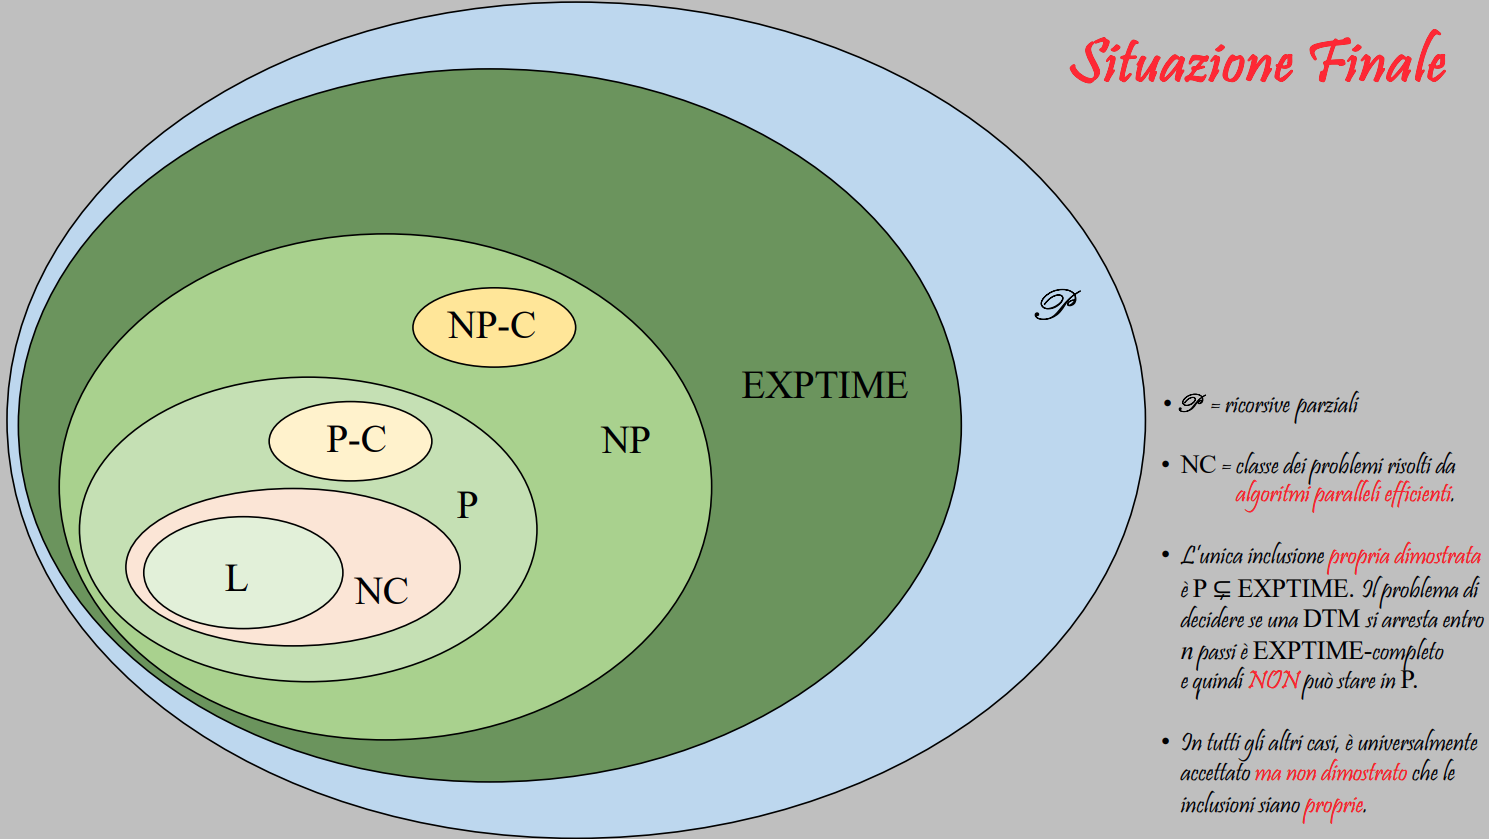
\includegraphics[width=1\textwidth]{img/finale.png}
\end{figure}


%%% Local Variables:
%%% TeX-master: "../it.tex"
%%% End:


\end{document}
